\documentclass[12pt,a4paper,oneside]{report}
\usepackage[utf8]{inputenc}
\usepackage[T1]{fontenc}
\usepackage[english]{babel}
\babelprovide[import,main]{brazilian}
\usepackage{mathptmx}
\usepackage[left=3cm,right=2cm,top=3cm,bottom=2cm,headheight=15pt,headsep=18pt]{geometry}
\usepackage{setspace,graphicx,float,tabularx,array,caption,titlesec,fancyhdr,xurl,indentfirst}
\usepackage[hidelinks,unicode]{hyperref}
\hypersetup{pdftitle={Prazo Claro --- Sistema de contagem de prazos processuais brasileiros},pdfauthor={Kezia Calixto},pdfsubject={Trabalho de Graduação II --- versão para revisão}}
\selectlanguage{brazilian}
\onehalfspacing
\setlength{\parindent}{1.25cm}
\setlength{\parskip}{0pt}
\setlength{\emergencystretch}{3em}
\titleformat{\chapter}[block]{\normalfont\bfseries\fontsize{14}{18}\selectfont}{\thechapter}{1em}{}
\titlespacing*{\chapter}{0pt}{0pt}{24pt}
\titleformat{\section}{\normalfont\bfseries\fontsize{12}{16}\selectfont}{\thesection}{1em}{}
\titlespacing*{\section}{0pt}{18pt}{12pt}
\DeclareCaptionFont{tgcaption}{\fontsize{10}{12}\selectfont}
\captionsetup{font={tgcaption,stretch=1},labelfont=normalfont,labelsep=endash,position=top}
\counterwithout{figure}{chapter}
\counterwithout{table}{chapter}
\floatstyle{plaintop}
\newfloat{quadro}{H}{loq}
\floatname{quadro}{Quadro}
\newcommand{\listquadros}{\listof{quadro}{LISTA DE QUADROS}}
\renewcommand{\contentsname}{SUMÁRIO}
\renewcommand{\listfigurename}{LISTA DE FIGURAS}
\renewcommand{\listtablename}{LISTA DE TABELAS}
\addto\captionsbrazilian{\renewcommand{\contentsname}{SUMÁRIO}\renewcommand{\listfigurename}{LISTA DE FIGURAS}\renewcommand{\listtablename}{LISTA DE TABELAS}}
\pagestyle{fancy}\fancyhf{}\fancyhead[R]{\fontsize{10}{12}\selectfont\thepage}
\renewcommand{\headrulewidth}{0pt}
\fancypagestyle{plain}{\fancyhf{}\fancyhead[R]{\fontsize{10}{12}\selectfont\thepage}\renewcommand{\headrulewidth}{0pt}}
\setcounter{tocdepth}{1}
\begin{document}
\renewcommand{\contentsname}{SUMÁRIO}
\renewcommand{\listfigurename}{LISTA DE FIGURAS}
\renewcommand{\listtablename}{LISTA DE TABELAS}
\pagestyle{empty}
\fancypagestyle{plain}{\fancyhf{}\renewcommand{\headrulewidth}{0pt}}
\hypersetup{pageanchor=false}
\begin{titlepage}\centering
{\bfseries CENTRO ESTADUAL DE EDUCAÇÃO TECNOLÓGICA PAULA SOUZA\par
FACULDADE DE TECNOLOGIA DE CAMPINAS\par
Curso de Análise e Desenvolvimento de Sistemas\par}
\vspace{2.3cm}
Kezia Calixto\par
\vfill
{\bfseries\fontsize{14}{20}\selectfont PRAZO CLARO\par
Sistema de contagem de prazos processuais brasileiros\par}
\vfill
Campinas --- SP\par 2026
\end{titlepage}
\setcounter{page}{1}
\hypersetup{pageanchor=true}
\thispagestyle{empty}
\begin{center}Kezia Calixto\end{center}
\vspace{2.2cm}
\begin{center}\bfseries\fontsize{14}{20}\selectfont PRAZO CLARO\par
Sistema de contagem de prazos processuais brasileiros\end{center}
\vspace{2cm}
\begin{flushright}\begin{minipage}{.54\textwidth}\begin{singlespace}
Trabalho de Graduação II apresentado à Faculdade de Tecnologia de Campinas, do Centro Estadual de Educação Tecnológica Paula Souza, como requisito parcial para obtenção do título de Tecnóloga em Análise e Desenvolvimento de Sistemas.\par\medskip
Orientador: Prof. Eduardo Felipe Fonseca de Freitas.
\end{singlespace}\end{minipage}\end{flushright}
\vfill
\begin{center}Versão para revisão da autora e do orientador\par
24 de outubro de 2026\par\vspace{1cm}Campinas --- SP\par 2026\end{center}
\clearpage
\chapter*{RESUMO}\thispagestyle{empty}
\begin{singlespace}\noindent A contagem de prazos processuais depende da identificação do evento comunicado, do regime aplicável e do calendário do órgão competente. Este trabalho apresenta a concepção, a implementação e a verificação do Prazo Claro, uma aplicação web acadêmica voltada à produção de estimativas explicáveis. O objetivo foi construir um motor determinístico com memória de cálculo, versões preservadas e integração a recursos privados de histórico e lembrete. O desenvolvimento utilizou análise documental, levantamento de fontes primárias, especificação incremental e testes em diferentes fronteiras. A solução separou o domínio de contagem da interface Next.js e dos serviços Supabase, adotou datas civis com Temporal e manteve regras e calendários versionados. O recorte implementado abrange perfis civis e criminais ordinários do TJSP em dez comarcas de São Paulo no exercício de 2026 e perfil trabalhista ordinário do TRT da 2\textordfeminine{} Região na Capital em 2026--2027. A verificação automatizada identificada registrou 256 testes unitários, 146 testes SQL e 67 cenários de navegador aprovados, com um cenário omitido. Os resultados incluem memória exportável, autenticação, histórico individual e agendamento opcional de lembretes. Calendários parciais, revisão jurídica pendente e recebimento externo ainda sujeito a aceite limitam o alcance da entrega. Conclui-se que o artefato atende ao recorte técnico documentado e oferece uma base rastreável para revisão e continuidade, sem constituir certificação de tempestividade ou cobertura universal de procedimentos.\par\medskip
\noindent\textbf{Palavras-chave:} Engenharia de software. Prazos processuais. Rastreabilidade. Aplicação web.
\end{singlespace}
\clearpage
\chapter*{ABSTRACT}\thispagestyle{empty}
\begin{otherlanguage}{english}\begin{singlespace}\noindent Procedural deadline calculation depends on identifying the communicated event, the applicable procedural rules, and the competent court's calendar. This work presents the conception, implementation, and verification of Prazo Claro, an academic web application designed to produce explainable estimates. The objective was to build a deterministic engine with a calculation record, preserved versions, and integration with private history and reminder features. Development combined documentary analysis, primary-source research, incremental specification, and tests across different system boundaries. The solution separated the calculation domain from the Next.js interface and Supabase services, used Temporal for calendar dates, and preserved versioned rules and calendars. The implemented scope includes ordinary civil and criminal profiles for ten TJSP localities in São Paulo in 2026 and an ordinary labor profile for the TRT of the 2nd Region in the city of São Paulo in 2026--2027. The identified automated verification recorded 256 unit tests, 146 SQL tests, and 67 browser scenarios passing, with one scenario skipped. Results include exportable calculation records, authentication, individual history, and optional reminder scheduling. Partial calendars, pending legal review, and external email receipt still requiring acceptance limit the delivery's scope. The artifact meets its documented technical scope and provides a traceable basis for review and further development, without certifying procedural timeliness or universal procedural coverage.\par\medskip
\noindent\textbf{Keywords:} Software engineering. Procedural deadlines. Traceability. Web application.
\end{singlespace}\end{otherlanguage}
\clearpage\listoffigures\thispagestyle{empty}
\clearpage\listquadros\thispagestyle{empty}
\clearpage\listoftables\thispagestyle{empty}
\clearpage\chapter*{LISTA DE ABREVIATURAS E SIGLAS}\thispagestyle{empty}
\begin{singlespace}\noindent
ADS --- Análise e Desenvolvimento de Sistemas\\
API --- Interface de programação de aplicações\\
AR --- Aviso de recebimento\\
CI --- Integração contínua\\
CLT --- Consolidação das Leis do Trabalho\\
CNJ --- Conselho Nacional de Justiça\\
CPC --- Código de Processo Civil\\
CPP --- Código de Processo Penal\\
DJEN --- Diário de Justiça Eletrônico Nacional\\
E2E --- Teste ponta a ponta\\
LGPD --- Lei Geral de Proteção de Dados Pessoais\\
PKCE --- Proof Key for Code Exchange\\
RLS --- Row Level Security\\
SSR --- Server-Side Rendering\\
TG --- Trabalho de Graduação\\
TJSP --- Tribunal de Justiça do Estado de São Paulo\\
TRT --- Tribunal Regional do Trabalho\\
WCAG --- Web Content Accessibility Guidelines
\end{singlespace}
\clearpage\tableofcontents\thispagestyle{empty}
\clearpage\pagestyle{fancy}
\fancypagestyle{plain}{\fancyhf{}\fancyhead[R]{\fontsize{10}{12}\selectfont\thepage}\renewcommand{\headrulewidth}{0pt}}
\chapter{INTRODUÇÃO}
\label{chapter-1}
\section{Contextualização}
\label{section-1-1}
A contagem de um prazo processual exige identificar o evento comunicado, a regra aplicável e o calendário do órgão competente. A data exibida no diário, a publicação juridicamente considerada e o primeiro dia computado podem ser diferentes. A mesma duração também pode produzir resultados distintos em localidades ou regimes diferentes. Essa combinação torna insuficiente uma calculadora que apenas some dias a uma data.

O Prazo Claro foi concebido como aplicação acadêmica para tornar essas decisões visíveis. A proposta reúne formulário orientado, motor determinístico, calendário versionado e memória de cálculo. O resultado permite examinar os marcos e o motivo de cada inclusão ou exclusão. O foco do Trabalho de Graduação II é a construção e a verificação de um artefato de software explicável, com documentação suficiente para sua continuidade.

O projeto originou-se dos documentos de concepção e do rascunho de TG preservados no repositório. Durante a implementação, a proposta foi delimitada para uma aplicação web responsiva, inicialmente civil e posteriormente ampliada a perfis criminais e trabalhistas expressos. As referências a aplicativo móvel, inteligência artificial em produção e funcionalidades ainda não construídas não são apresentadas como resultados alcançados. Essa distinção entre intenção e implementação orienta todo o relatório.

\section{Problema e justificativa}
\label{section-1-2}
A questão de desenvolvimento foi formulada da seguinte maneira: como construir uma aplicação que produza estimativas processuais reproduzíveis e apresente seus fundamentos e limitações, sem ocultar a dependência de regras e calendários locais? A questão envolve tanto a operação de contagem quanto o tratamento de entradas incompletas, a preservação histórica e a comunicação de incerteza.

Uma data final isolada não permite verificar se o sistema selecionou a comarca correta, confundiu disponibilização com publicação ou aplicou indevidamente uma suspensão. Por isso, a justificativa técnica do projeto está na rastreabilidade: registrar as premissas e as versões utilizadas torna possível investigar divergências e comparar resultados após mudanças de catálogo. O software também oferece um objeto concreto para estudar requisitos, modelagem, segurança e testes em um domínio no qual erros têm consequências relevantes.

O Código de Processo Civil, a legislação trabalhista e o Código de Processo Penal possuem dispositivos próprios sobre contagem e suspensão. A existência desses dispositivos fundamenta a separação de perfis adotada no projeto; não autoriza aplicar uma única opção de dias úteis ou corridos a qualquer procedimento. A demonstração acadêmica conserva a necessidade de conferência profissional e de documentação da comunicação efetivamente ocorrida \hyperref[ref:CPC]{(BRASIL, 2015)} \hyperref[ref:CLT]{(BRASIL, 1943)} \hyperref[ref:CPP]{(BRASIL, 1941)}.

\section{Objetivos}
\label{section-1-3}
O objetivo geral foi desenvolver e verificar uma aplicação web de contagem processual com memória explicável, versões preservadas e serviços privados de histórico e lembrete, dentro de recortes declarados do Estado de São Paulo.

Os objetivos específicos foram: (1) especificar requisitos e modelos que distinguissem comunicação, contagem, fontes e cobertura; (2) implementar um motor independente da interface e integrá-lo à aplicação, à autenticação e à persistência com autorização; e (3) verificar o comportamento por casos de referência e testes em diferentes fronteiras, documentando resultados, limitações e procedimentos de entrega.

\section{Delimitação e organização}
\label{section-1-4}
O recorte civil contempla processo comum, TJSP, dez comarcas cadastradas, exercício de 2026, comunicação pelo diário e contagem em dias úteis. O criminal contempla contexto ordinário confirmado nessas mesmas comarcas e ano, com início e prorrogação próprios. O trabalhista contempla exclusivamente TRT da 2\textordfeminine{} Região, município de São Paulo, contexto ordinário e calendários de 2026 e 2027. A escolha do suporte físico ou eletrônico dos autos não transforma o diário em comunicação pessoal.

Os calendários são demonstrativos e parciais, com revisão jurídica profissional pendente. Não há suporte geral a todo o Estado, a todos os procedimentos ou a qualquer prazo brasileiro. Permanecem excluídos, entre outros, TRT-15, TJSP 2027, juizados, procedimentos especiais, prazo material penal, horas, meses, anos, prazo em dobro e comunicações por AR, mandado ou Domicílio Judicial Eletrônico.

O relatório apresenta fundamentos, método, concepção, implementação e resultados. Os apêndices detalham casos de uso, dados, API, rastreabilidade e procedimentos de continuidade. A base funcional descrita é o commit 9632fd2. O corte documental é 24 de outubro de 2026: resultados posteriores precisam de nova evidência e não são presumidos neste texto.

\chapter{FUNDAMENTAÇÃO E TRABALHOS DE REFERÊNCIA}
\label{chapter-2}
\section{Engenharia de software e requisitos}
\label{section-2-1}
O SWEBOK organiza conhecimentos de engenharia de software, incluindo requisitos, arquitetura e testes. A edição consultada é a versão 4.0a, cuja capa registra lançamento em agosto de 2026. Neste trabalho, essa referência apoiou a organização das atividades e dos artefatos, sem impor a adoção integral de um processo específico \hyperref[ref:SWEBOK]{(IEEE COMPUTER SOCIETY, 2026)}. A passagem da proposta ampla para critérios verificáveis foi uma decisão do projeto: cada funcionalidade recebeu um recorte, uma condição de aceite e uma evidência esperada.

A especificação diferencia requisitos funcionais, atributos de qualidade e regras de negócio. Calcular, salvar e cancelar um lembrete são comportamentos observáveis; determinismo e controle de acesso são condições transversais. Uma norma jurídica não é tratada como requisito completo por si só: sua implementação depende de âmbito, vigência, condições de aplicação e casos de referência. A matriz de rastreabilidade estabelece as relações entre esses elementos no artefato construído.

O resumo público da ISO/IEC 25010:2023 apresenta um modelo de qualidade de produto composto por nove características. A referência foi usada como orientação para discutir qualidade, não como certificação ou avaliação integral da norma. O texto completo pago não foi utilizado como se tivesse sido integralmente examinado \hyperref[ref:ISO25010]{(ISO; IEC, 2023)}. No Prazo Claro, os critérios efetivamente verificados foram registrados por teste ou observação, sem atribuir pontuações globais de qualidade.

\section{Comunicação, calendário e contagem}
\label{section-2-2}
A Lei 11.419/2006 distingue a disponibilização no diário da data considerada de publicação e trata do início de prazos decorrentes desse meio. O CPC contém regras sobre dias úteis, suspensão e exclusão do dia do começo. Esses conceitos foram separados no contrato do motor para evitar o uso de um campo genérico de data inicial \hyperref[ref:LEI11419]{(BRASIL, 2006)} \hyperref[ref:CPC]{(BRASIL, 2015)}. A regulamentação do CNJ sobre DJEN e Domicílio, com a alteração da Resolução 569/2024, reforça a necessidade de distinguir os meios de comunicação; o sistema implementa apenas o perfil de diário especificado \hyperref[ref:CNJ569]{(CNJ, 2024)}.

No perfil criminal, a pesquisa do projeto examinou os arts. 798 e 798-A do CPP e preservou a distinção entre o fim nominal e a eventual prorrogação. No trabalhista, examinou os arts. 775 e 775-A da CLT. O catálogo inicial de atos inclui apelação civil, recurso ordinário trabalhista da Vara do Trabalho e declaração de sentença penal de primeiro grau. Cada seleção exige confirmação das condições específicas; não decide admissibilidade, tempestividade real ou efeitos de um recurso sobre outro prazo \hyperref[ref:CPP]{(BRASIL, 1941)} \hyperref[ref:CLT]{(BRASIL, 1943)} \hyperref[ref:CPC]{(BRASIL, 2015)}.

O calendário constitui dado normativo e operacional versionado. A relação municipal do TJSP para 2026 e os atos forenses usados pelo projeto possuem âmbito e período próprios. A Portaria GP 19/2026 do TRT-2 fundamenta eventos de 2027 naquele tribunal. A presença dessa fonte não preenche a lacuna de outro tribunal ou comarca \hyperref[ref:TJSPMUN]{(TJSP, 2025a)} \hyperref[ref:TJSP2813]{(TJSP, 2025b)} \hyperref[ref:TRT2027]{(TRT-2, 2026)}. As fichas do repositório conservam dispositivo, consulta, vigência e estado de revisão de cada seleção.

\section{Datas civis e reprodutibilidade}
\label{section-2-3}
A documentação de Temporal.PlainDate descreve uma data de calendário independente de fuso horário. Esse conceito foi adotado para os eventos processuais e para as datas percorridas pelo motor \hyperref[ref:TEMPORAL]{(TC39, s.d.)}. Um vencimento em 27 de outubro é armazenado como data civil; não é convertido implicitamente em meia-noite UTC. Já o envio de um lembrete exige um instante associado ao horário escolhido em America/Sao\_Paulo.

Reprodutibilidade, neste projeto, significa executar a mesma entrada com as mesmas versões e obter a mesma memória. Não significa que o resultado esteja juridicamente aprovado nem que um JSON salvo seja autêntico. A implementação preserva cópias dos dados utilizados, identifica motores anteriores e separa uma recomputação possível do snapshot original. Essa separação permite reconhecer versões indisponíveis sem substituir a evidência histórica por um cálculo atual.

\section{Arquitetura web e persistência}
\label{section-2-4}
Os Route Handlers do Next.js permitem implementar endpoints HTTP na aplicação. O projeto utilizou essa capacidade para separar contratos de cálculo, conta, histórico e lembretes, mantendo o algoritmo fora do framework \hyperref[ref:NEXT]{(VERCEL, s.d.)}. A escolha de monólito modular reduz a quantidade de serviços operados nesta entrega e conserva fronteiras que podem ser testadas isoladamente.

A documentação de Supabase apresenta clientes distintos para contexto de navegador e servidor em integrações SSR e o uso de políticas PostgreSQL de segurança por linha. Essas capacidades fundamentam a infraestrutura escolhida \hyperref[ref:SUPABASESSR]{(SUPABASE, s.d.a)} \hyperref[ref:SUPABASERLS]{(SUPABASE, s.d.b)}. No sistema desenvolvido, a identidade é verificada no servidor, e a autorização do histórico também é expressa no banco. Uma resposta visual de conectado não é a única barreira para acessar dados privados.

\section{Segurança, privacidade e acessibilidade}
\label{section-2-5}
O ASVS da OWASP oferece requisitos para verificação de segurança de aplicações. A referência consultada foi a versão estável 5.0.0; o projeto utilizou preocupações como validação e autorização para organizar sua análise, sem declarar conformidade integral \hyperref[ref:ASVS]{(OWASP, 2025)}. Os controles efetivamente existentes são descritos na implementação e nos testes. Não houve auditoria independente nem ensaio amplo de resistência a abuso.

A LGPD fundamenta a atenção à finalidade, à necessidade e à proteção dos dados pessoais. O artefato evita exigir nomes de partes e números de processos para realizar cálculos; conta e e-mail são necessários aos recursos privados escolhidos. Esta documentação não substitui uma definição institucional de controlador, retenção, atendimento e base legal para eventual operação ampliada \hyperref[ref:LGPD]{(BRASIL, 2018)}.

A WCAG 2.2 reúne critérios verificáveis de acessibilidade. Foi adotada como meta de nível AA, com foco em teclado, rótulos, mensagens de erro e percepção de estados \hyperref[ref:WCAG]{(W3C, 2024)}. Verificações automatizadas e inspeções de telas foram registradas, mas não abrangem todos os critérios nem equivalem a uma certificação. A avaliação com pessoas usuárias de tecnologias assistivas permanece como evolução.

\chapter{MATERIAIS E MÉTODO DE DESENVOLVIMENTO}
\label{chapter-3}
\section{Natureza e fontes do trabalho}
\label{section-3-1}
O trabalho teve natureza aplicada, com desenvolvimento de um artefato de software e análise documental. O material de partida incluiu o master prompt, os rascunhos acadêmicos e os demais arquivos recebidos em docs. O manual de TG da FATEC Campinas, edição de maio de 2024, e o template institucional orientaram a organização desta documentação \hyperref[ref:FATECMANUAL]{(FATEC CAMPINAS, 2024)}. Os originais foram preservados, e as divergências da proposta foram registradas separadamente.

O levantamento técnico utilizou o código, migrations, testes, registros de execução, decisões arquiteturais e documentos de operação do próprio projeto. O levantamento normativo utilizou fontes primárias, com fichas locais de consulta. Reuniões, entrevistas, amostragem de profissionais e pesquisa de satisfação não foram realizadas como parte do conjunto de evidências aqui apresentado. Os perfis de usuário descritos são analíticos, derivados das necessidades do produto, e não personas validadas por pesquisa de campo.

\section{Procedimento incremental}
\label{section-3-2}
A sequência de trabalho consistiu em revisar a concepção, estabilizar um vocabulário, definir uma primeira fatia civil e implementar motor, interface e memória. Em seguida, foram integrados conta e histórico privado; a cobertura municipal e os perfis criminal e trabalhista receberam especificação própria. A composição de calendários anuais, o catálogo inicial de atos e os lembretes foram incorporados em marcos posteriores. Cada avanço ficou identificável no Git e nos documentos de verificação.

Nas regras de negócio, adotou-se a sequência caso e fonte, teste inicialmente falho, implementação e regressão. Nos serviços de integração, as fronteiras de teste foram escolhidas conforme o risco: funções puras, contratos HTTP, políticas SQL, navegador e integração real local. O processo foi incremental; não há registro suficiente para descrevê-lo como uma aplicação completa de Scrum, com sprints, cerimônias e métricas formais.

Ferramentas de assistência por IA apoiaram programação, pesquisa documental e preparação dos materiais. O produto publicado não depende de modelo de linguagem para calcular datas. A autora e a orientação devem revisar o conteúdo, a aderência às regras acadêmicas de autoria e a declaração institucional de uso dessas ferramentas antes da submissão. O texto não atribui a participantes entrevistas, avaliações ou aprovações inexistentes.

\section{Ambiente e instrumentos}
\label{section-3-3}
O ambiente local utilizou Windows, Node.js da linha 22 a partir de 22.14, pnpm 11.0.8 e Docker Desktop. As versões declaradas no package.json incluem Next.js 16.4.2, React 19.3.1, TypeScript 6.0.3 e Supabase CLI 2.121.0. O lockfile fixa a resolução de dependências. A integração contínua também executa em Linux, evitando apresentar Windows como único ambiente possível.

Vitest e fast-check apoiam testes de unidades e propriedades; Playwright e Axe apoiam navegação e acessibilidade automatizada; pgTAP verifica políticas e funções SQL. Supabase local fornece banco, Auth e Mailpit para mensagens de teste. GitHub Actions executa verificações, Vercel hospeda a aplicação e Supabase hospeda os serviços de dados e identidade. O Brevo foi configurado para SMTP de autenticação e, separadamente, para a API de lembretes.

\section{Critérios de verificação e corte de evidências}
\label{section-3-4}
Um requisito técnico foi considerado verificado apenas quando houve execução ou observação identificada. Arquivos de configuração não foram tratados como prova de integração. Testes com respostas simuladas no navegador verificam interação, enquanto cadastro, cookies, persistência e isolamento exigem serviços reais. O aceite de uma mensagem pelo provedor também foi separado do recebimento pelo destinatário.

O registro consolidado usa a CI 40061653068 da versão funcional 9632fd2. As verificações locais e hospedadas possuem documentos próprios em docs/testing \hyperref[ref:PROJETO]{(PRAZO CLARO, 2026)}. A elaboração deste relatório não executou uma nova pesquisa de usuários nem repetiu toda a bateria do aplicativo. Os números apresentados pertencem aos registros identificados, e a análise de limitações considera essa origem.

\chapter{CONCEPÇÃO E ENGENHARIA DO SISTEMA}
\label{chapter-4}
\section{Evolução da proposta e partes interessadas}
\label{section-4-1}
A concepção inicial pretendia oferecer apoio à contagem de prazos em diferentes ramos e ambientes. A revisão identificou que calendário, comunicação e exceções impediam tratar o objetivo amplo como uma única fórmula. A primeira decisão foi reduzir o escopo de implementação sem apagar o objetivo original. O backlog conserva expansões, enquanto cada perfil entregue declara suas condições.

As partes interessadas consideradas são a autora, a orientação, a banca, a pessoa que realiza a simulação e o responsável técnico pela instalação. Um profissional de Direito é necessário à revisão jurídica futura, mas sua aprovação não consta como concluída. O usuário anônimo pode calcular e consultar fontes; o autenticado pode manter o próprio histórico e solicitar lembretes. Administração normativa e trabalho em equipe não são papéis funcionais implementados.

\section{Escopo funcional e requisitos}
\label{section-4-2}
O quadro a seguir sintetiza o contrato efetivamente implementado. Os identificadores RF e RNF mantêm relação com docs/requirements.md; os limites dos perfis e os contratos posteriores complementam o documento histórico da primeira fatia.

\begin{quadro}[H]\centering
\caption{Requisitos funcionais do recorte entregue}
\label{quadro-1}
\begin{singlespace}\fontsize{10}{12}\selectfont
\begin{tabularx}{\linewidth}{|>{\raggedright\arraybackslash}X|>{\raggedright\arraybackslash}X|}
\hline
\textbf{ID} & \textbf{Comportamento verificável} \\
\hline
RF01 & Distinguir disponibilização e publicação no diário; identificar a data solicitada. AR e mandado permanecem fora do recorte. \\
\hline
RF02 & Aplicar a contagem do perfil selecionado, com marco excluído e primeiro dia computado separados. \\
\hline
RF03 & Selecionar calendário por tribunal, município e versão, conservando fontes dos eventos. \\
\hline
RF04 & Exibir marcos, trilha diária, motivo das decisões e vencimento quando determinável. \\
\hline
RF05 & Produzir estado incompleto e vencimento nulo quando faltar cobertura ou enquadramento. \\
\hline
RF06 & Exportar JSON e imprimir a memória com versões, avisos e fontes. \\
\hline
RF07 & Autenticar, salvar, listar e excluir somente cálculos da própria conta. \\
\hline
RF08 & Consultar calendários e fontes; não oferecer administração normativa remota. \\
\hline
RF09 & Agendar e cancelar lembrete opcional, com consentimento, fuso e situação de envio explícitos. \\
\hline
\end{tabularx}\end{singlespace}
\par\smallskip{\fontsize{10}{12}\selectfont Fonte: elaboração com base nos registros do projeto (2026).}
\end{quadro}
\begin{quadro}[H]\centering
\caption{Requisitos de qualidade e sua expressão no projeto}
\label{quadro-2}
\begin{singlespace}\fontsize{10}{12}\selectfont
\begin{tabularx}{\linewidth}{|>{\raggedright\arraybackslash}X|>{\raggedright\arraybackslash}X|}
\hline
\textbf{ID} & \textbf{Decisão e critério} \\
\hline
RNF01 & Motor determinístico, independente de rede, banco, React e relógio do sistema. \\
\hline
RNF02 & Datas civis em ISO/PlainDate; instantes de envio com fuso explícito de São Paulo. \\
\hline
RNF03 & Interface responsiva em pt-BR, erros associados, teclado e foco visível; WCAG AA como meta. \\
\hline
RNF04 & Validação e identidade no servidor, RLS, segredos fora do navegador e minimização de dados. \\
\hline
RNF05 & Versões e snapshots preservados; recomputação separada do original. \\
\hline
RNF06 & Tipos, lint, formatação, testes, build e migrations verificáveis por execução. \\
\hline
RNF07 & Hospedagem em Vercel e serviços Supabase integrados por ambiente. \\
\hline
\end{tabularx}\end{singlespace}
\par\smallskip{\fontsize{10}{12}\selectfont Fonte: elaboração com base nos registros do projeto (2026).}
\end{quadro}
As regras transversais exigem fonte primária e estado de revisão, recusam incompatibilidade territorial e temporal e preservam a indicação de demonstração. Calendário ausente não é substituído pelo de outra comarca. Contexto desconhecido não é convertido em ordinário. O servidor não recebe do navegador um calendário livre nem confia em um vencimento informado pelo cliente para salvar o histórico.

\section{Casos de uso e fluxo principal}
\label{section-4-3}
O fluxo público compreende selecionar perfil e localidade, identificar a comunicação, informar data e duração, calcular e examinar a memória. O fluxo privado acrescenta entrar, salvar, consultar, exportar ou excluir. O lembrete nasce de um cálculo salvo elegível e exige escolha expressa. Os casos de uso detalhados no Apêndice A registram precondições e alternativas, evitando descrever somente o caminho de sucesso.

\begin{figure}[H]\centering
\caption{Contexto e recursos disponíveis ao usuário}
\label{figure-1}
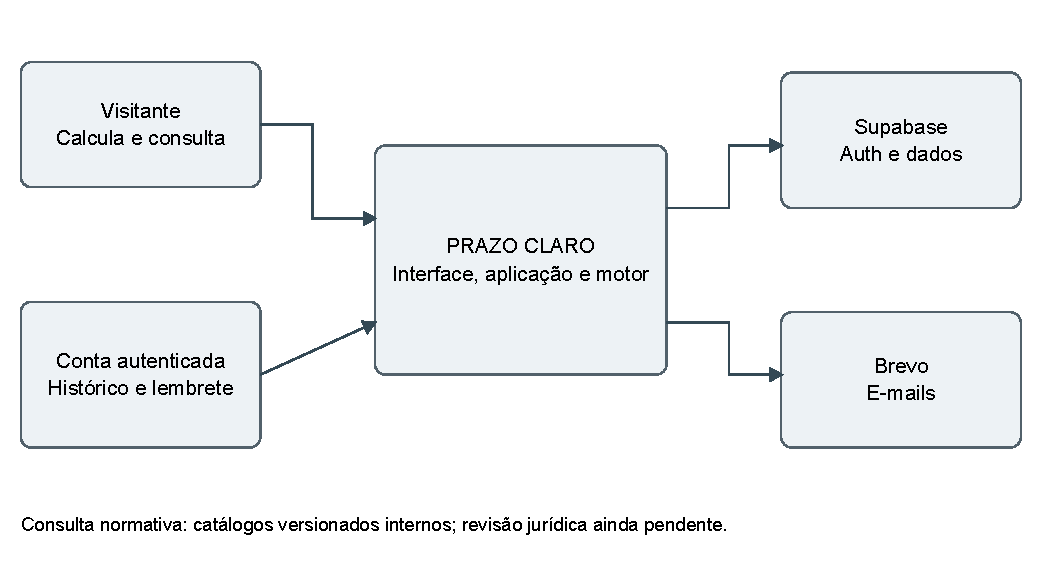
\includegraphics[width=\linewidth,height=.49\textheight,keepaspectratio]{figuras/contexto.pdf}
\par\smallskip{\fontsize{10}{12}\selectfont Fonte: elaboração para este relatório a partir do código e da documentação do Prazo Claro (2026).}
\end{figure}
As fronteiras externas da figura são reais: Supabase participa da identidade e dos dados, e Brevo participa das mensagens. A contagem pública não exige autenticação nem consulta remota durante a execução do motor. A indisponibilidade da configuração de conta é exibida sem apresentar uma sessão fictícia.

\section{Modelo de domínio}
\label{section-4-4}
O vocabulário distingue regime, perfil, suporte dos autos, meio de comunicação, evento, publicação, primeiro dia computado, fim nominal e vencimento. Uma regra versionada define o método dentro de um âmbito. O calendário versionado contém eventos e fontes. A entrada referencia as condições de seleção, e o resultado conserva trilha e cópias dos dados utilizados. Essas entidades lógicas não correspondem necessariamente a tabelas separadas.

\begin{figure}[H]\centering
\caption{Modelo conceitual de cálculo e memória}
\label{figure-2}
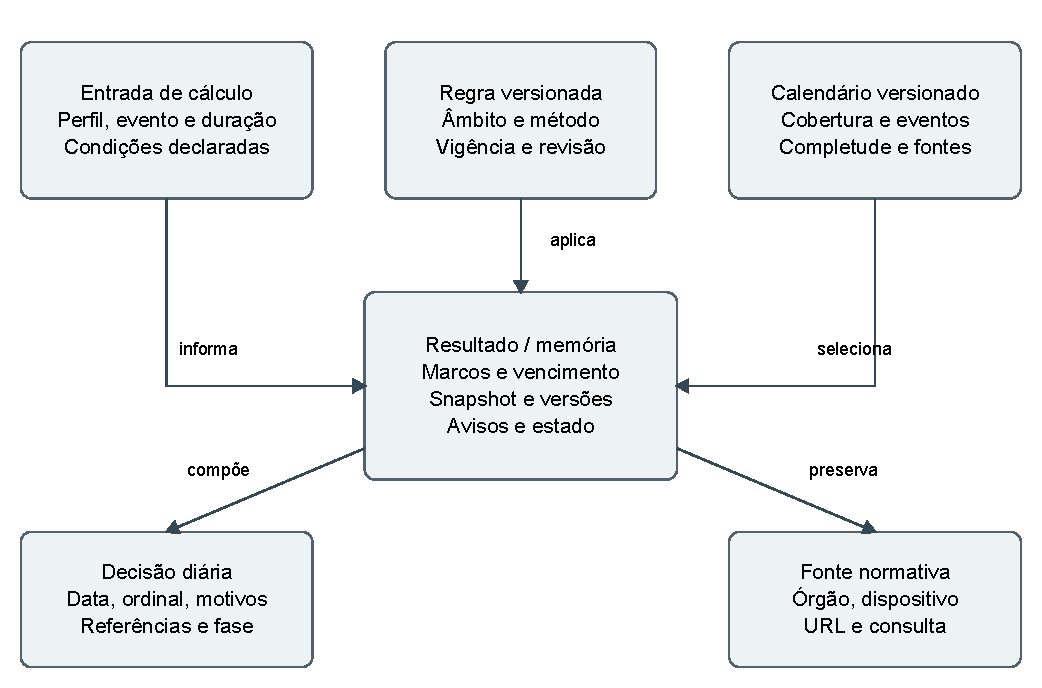
\includegraphics[width=\linewidth,height=.49\textheight,keepaspectratio]{figuras/dominio.pdf}
\par\smallskip{\fontsize{10}{12}\selectfont Fonte: elaboração para este relatório a partir do código e da documentação do Prazo Claro (2026).}
\end{figure}
A trilha é composta por decisões datadas: a data pode ser contada ou excluída, recebe ordinal quando consome unidade e conserva motivos e referências. O perfil criminal pode acrescentar uma fase de prorrogação sem consumir novas unidades. A memória mantém ainda pendências e estado de revisão, para que a exportação não transforme uma estimativa demonstrativa em resultado aprovado.

\section{Arquitetura e decisões}
\label{section-4-5}
A aplicação adota monólito modular. A apresentação reúne páginas e componentes React; a camada de aplicação valida contratos e seleciona dados; o domínio executa a contagem; adaptadores integram Supabase, e-mail e infraestrutura. Os catálogos normativos ativos são arquivos TypeScript versionados. As tabelas de catálogos do banco existem no schema, mas não constituem uma administração remota completa nem substituem a seleção utilizada pelo motor.

\begin{figure}[H]\centering
\caption{Camadas e dependências da implementação}
\label{figure-3}
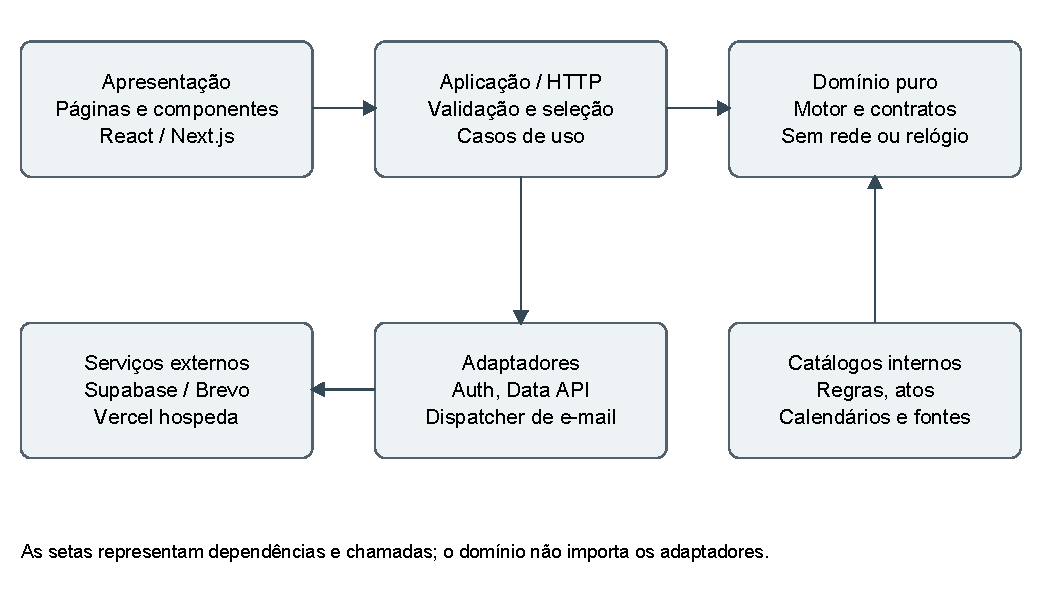
\includegraphics[width=\linewidth,height=.49\textheight,keepaspectratio]{figuras/arquitetura.pdf}
\par\smallskip{\fontsize{10}{12}\selectfont Fonte: elaboração para este relatório a partir do código e da documentação do Prazo Claro (2026).}
\end{figure}
Os ADRs registram seis decisões: motor independente e versões preservadas; Data API sem ORM inicial; histórico individual antes de organizações; novos perfis sem alterar o motor civil congelado; fila com tratamento de envio incerto; e agendamento com assinatura descartável. Não foram criados serviços NestJS ou um monorepo apenas para corresponder à proposta inicial. Uma separação futura depende de necessidade operacional demonstrada.

\section{Modelo físico e persistência}
\label{section-4-6}
O banco possui cinco tabelas públicas da aplicação: legal\_sources, legal\_rule\_versions, calendar\_versions, deadline\_calculations e deadline\_reminders. O schema reminder\_private contém configuração e invocações do agendador e funções internas. auth.users é gerenciada pelo Supabase Auth. Não existem tabelas públicas de organizações, membros, processos ou perfis administrativos neste recorte.

\begin{figure}[H]\centering
\caption{Relações físicas essenciais do banco}
\label{figure-4}
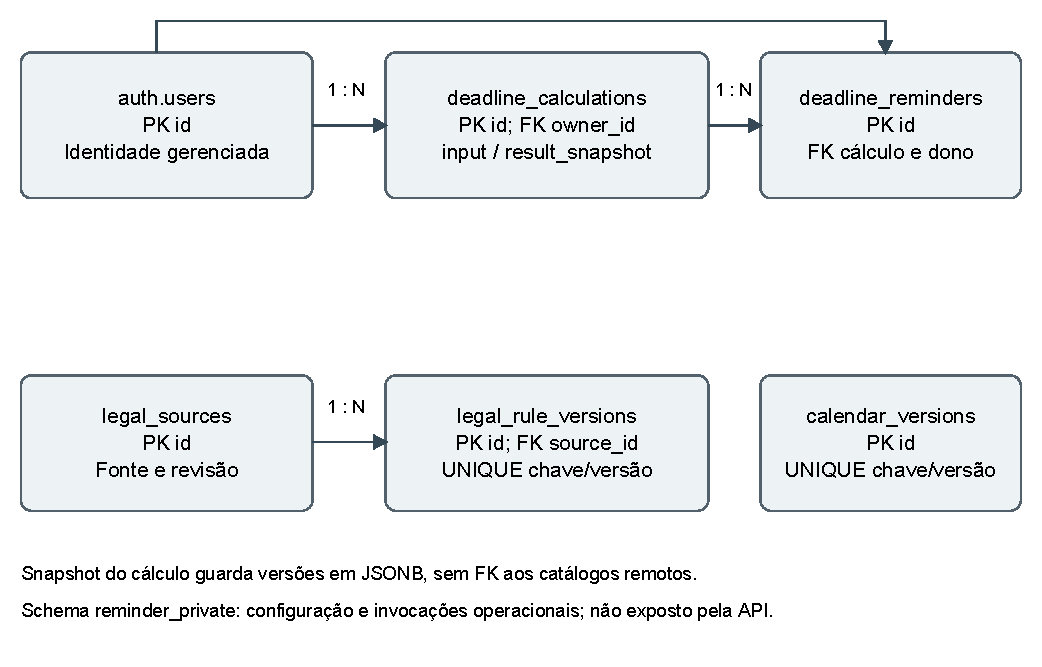
\includegraphics[width=\linewidth,height=.49\textheight,keepaspectratio]{figuras/dados.pdf}
\par\smallskip{\fontsize{10}{12}\selectfont Fonte: elaboração para este relatório a partir do código e da documentação do Prazo Claro (2026).}
\end{figure}
deadline\_calculations mantém proprietário, entrada e resultado em JSONB. O vínculo com versões normativas é preservado no snapshot; não existe uma chave estrangeira do cálculo para cada catálogo remoto. deadline\_reminders referencia cálculo e proprietário, com exclusão em cascata. Assim, apagar o cálculo remove o lembrete correspondente: essa consequência precisa ser compreendida antes de um ensaio de entrega.

Quatro migrations descrevem a evolução: 20261020001602 cria histórico e catálogos; 20261023172741 cria lembretes; 20261023184137 separa os modos de entrega; 20261023192044 instala o agendador. O dicionário do Apêndice B explicita campos e restrições. Atualizações usam migrations pendentes; reset de banco não é procedimento de manutenção de dados reais.

\section{Interface e experiência de uso}
\label{section-4-7}
O sistema utiliza um design system documentado, tipografia e espaçamento consistentes, campos rotulados e mensagens próximas à ação. A troca de perfil redefine escolhas incompatíveis. O ato opcional apresenta duração somente para leitura e exige confirmação específica; a quantidade manual permanece disponível. O resultado organiza data estimada, marcos, avisos, trilha e fontes, em vez de ocultar o contexto em uma nota genérica.

No histórico, o filtro por regime antecede a paginação no servidor. A busca textual é identificada como restrita à página atual. A situação futuro, hoje, passado ou indeterminado compara o vencimento original com a data de referência da aplicação, sem alterar o snapshot e sem afirmar cumprimento do ato. Estados vazios, carregamento, falha e exclusão possuem mensagens próprias.

Após cadastro aceito, uma página específica orienta a confirmar o e-mail no mesmo navegador, verificar spam e retornar ao acesso. Sua mensagem neutra evita revelar a existência de uma conta. A melhoria respondeu a um relato real: o e-mail chegava, mas a orientação permanecia no formulário. O contrato de confirmação e a proteção da sessão foram preservados.

\section{Segurança e tratamento de dados}
\label{section-4-8}
A identidade usada no servidor é obtida por verificação do usuário, e não por um ID confiado ao corpo da requisição. Políticas RLS restringem o histórico e a leitura de lembretes ao proprietário. Mutação privada confere origem e valida JSON. Chaves privilegiadas são exclusivas de código de servidor; a chave publicável e a existência de um botão oculto não substituem autorização.

Os fluxos de cadastro e recuperação apresentam mensagens genéricas. O callback troca código por sessão e restringe destinos. O fluxo de convite trata o retorno e permite definir senha; tokens e links de autenticação não integram logs ou documentação de entrega. Não são fornecidos arquivos privados .env, credenciais do Vault ou senhas ao pacote fonte.

RLS controla quem acessa uma linha, mas não comprova a autenticidade de uma memória inserida pelo próprio proprietário pela Data API. O histórico, portanto, identifica o snapshot como não verificado. Assinatura de memória, auditoria independente, controle distribuído de abuso, retenção institucional e restauração ensaiada permanecem fora da conclusão técnica deste recorte.

\chapter{IMPLEMENTAÇÃO E VERIFICAÇÃO}
\label{chapter-5}
\section{Organização do código e contratos}
\label{section-5-1}
O domínio de prazos fica em src/domain/deadlines; regras, atos e calendários possuem catálogos próprios. src/application concentra validação e seleção. Os Route Handlers de src/app/api implementam as fronteiras HTTP. O contrato público POST /api/calculate retorna diretamente CalculationResult; não persiste. O histórico e o agendamento exigem sessão, com autorização no servidor e no banco.

O schema recusa campos desconhecidos e combinações incompatíveis. Data impossível e corpo excessivo são erros de entrada/transporte; cobertura insuficiente é um resultado de domínio incompleto. Essa distinção orienta tanto a interface quanto os testes. O Apêndice C detalha parâmetros, códigos e exemplos sem conter credenciais reais.

\section{Algoritmo de contagem e composição}
\label{section-5-2}
A execução primeiro valida entrada, âmbito e versões. Se houver ato selecionado, verifica condições e duração antes de delegar a contagem. A comunicação pelo diário é normalizada para a publicação considerada; o marco excluído e o primeiro dia computado são registrados separadamente. O percurso avança por datas civis, avalia os efeitos normativos e do calendário e registra cada decisão até consumir a duração ou encontrar um impedimento.

\begin{figure}[H]\centering
\caption{Fluxo de decisão do cálculo demonstrativo}
\label{figure-5}
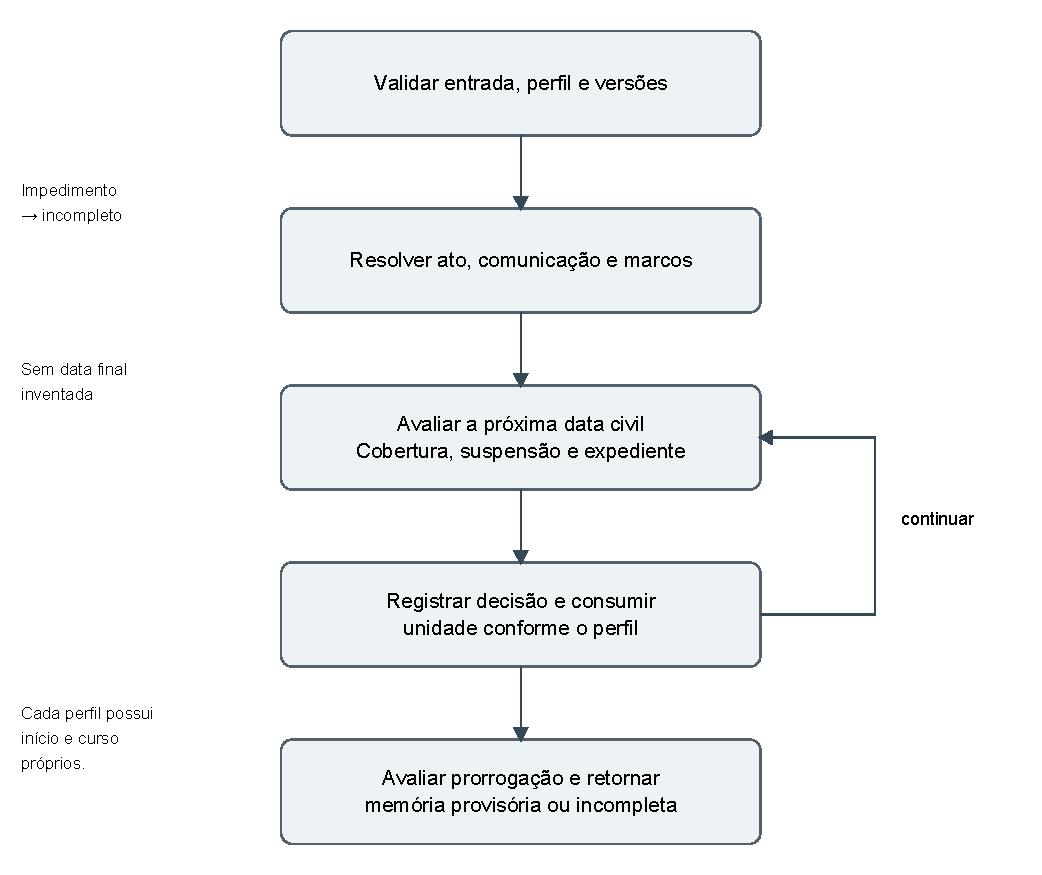
\includegraphics[width=\linewidth,height=.49\textheight,keepaspectratio]{figuras/calculo.pdf}
\par\smallskip{\fontsize{10}{12}\selectfont Fonte: elaboração para este relatório a partir do código e da documentação do Prazo Claro (2026).}
\end{figure}
O pseudocódigo descreve a organização, e não substitui as diferenças internas dos perfis:

\begin{quote}\begin{singlespace}\raggedright\ttfamily\footnotesize
\hspace*{0.0em}validar entrada e selecionar versões compatíveis\\
\hspace*{0.0em}se ato informado: verificar condições e duração\\
\hspace*{0.0em}determinar comunicação e marco inicial do perfil\\
\hspace*{0.0em}para cada data civil necessária:\\
\hspace*{2.0em}se cobertura/condição insuficiente: retornar incompleto\\
\hspace*{2.0em}avaliar início, suspensão, expediente e contagem\\
\hspace*{2.0em}registrar data, motivos, fontes e ordinal aplicável\\
\hspace*{2.0em}consumir unidade somente quando o perfil determinar\\
\hspace*{0.0em}se houver fim nominal: avaliar prorrogação própria\\
\hspace*{0.0em}retornar memória com versões, avisos e vencimento possível\\
\end{singlespace}\end{quote}
O motor civil 0.2.0 foi preservado. Os perfis ordinários criminal e trabalhista utilizam 0.3.0; a camada de composição de atos identifica 0.4.0 e informa também a versão da contagem delegada. Uma alteração de catálogo não reescreve uma versão anterior. Na travessia trabalhista, a aplicação tenta inicialmente o calendário anual existente e compõe 2026--2027 somente quando o percurso alcança o fim da cobertura e os componentes são compatíveis e contíguos.

Publicação, contagem e prorrogação não usam um único predicado genérico de dia útil. Um dia sem expediente e uma suspensão do curso do prazo podem produzir efeitos diferentes conforme a fase. A composição recusa lacunas, sobreposição, composição aninhada e eventos duplicados. Quando a informação não permite continuar, o sistema mantém dueDate nulo e informa as pendências em todos os formatos.

\section{Memória, exportação e histórico}
\label{section-5-3}
A memória contém entrada normalizada, evento, publicação, início, primeiro dia computado, fim nominal quando aplicável, vencimento, trilha, fontes e metadados. snapshot.calendar preserva cobertura e eventos; snapshot.rule e snapshot.act aparecem conforme o perfil. Componentes anuais ficam identificados quando há composição. O JSON e a impressão conservam os avisos demonstrativos.

Salvar no histórico envia a entrada e o título opcional ao servidor, que calcula novamente sob os catálogos internos. Não se aceita um vencimento do navegador como autoridade. Na leitura, o original é validado estruturalmente e permanece separado da recomputação. Quando a versão necessária não pode ser reexecutada, recomputed permanece nulo e o usuário conserva acesso ao original legível.

Paginação e filtro são aplicados com proprietário fixo, ordem por created\_at e id e tamanho limitado. A exclusão atualiza os totais da interface e trata a última página esvaziada. Títulos devem ser fictícios na demonstração, porque o campo livre pode conter dados que o sistema não precisa para contar.

\section{Conta e autenticação}
\label{section-5-4}
E-mail e senha, convite, recuperação e Google foram integrados ao Supabase Auth. Cadastro e recuperação usam confirmação por mensagem e retorno controlado. A troca PKCE utiliza o mesmo contexto de navegador para validar o retorno. O indicador de conectado permite perceber a sessão, e os recursos privados continuam verificando identidade em cada operação relevante.

\begin{figure}[H]\centering
\caption{Confirmação de cadastro e criação de sessão}
\label{figure-6}
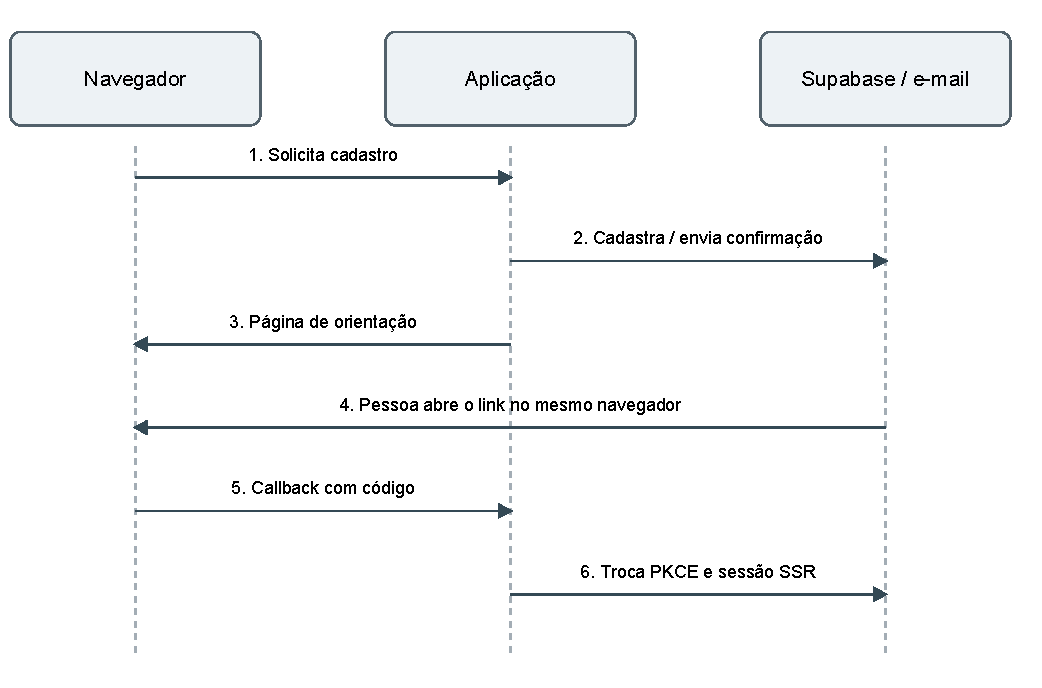
\includegraphics[width=\linewidth,height=.49\textheight,keepaspectratio]{figuras/autenticacao.pdf}
\par\smallskip{\fontsize{10}{12}\selectfont Fonte: elaboração para este relatório a partir do código e da documentação do Prazo Claro (2026).}
\end{figure}
A configuração de Site URL e de destinos permitidos no Supabase participa do retorno dos e-mails. Ela é diferente das URLs autorizadas no cliente Google. Os templates locais do CLI também não atualizam automaticamente o projeto hospedado. Essa distinção foi registrada durante a integração, pois receber a mensagem, abrir o destino e obter uma sessão são etapas diferentes.

\section{Lembretes e concorrência}
\label{section-5-5}
O lembrete é opcional e associado a um cálculo salvo elegível. A pessoa escolhe zero, um ou três dias corridos de antecedência e 09h, 12h ou 18h no fuso de São Paulo. Essa antecedência não altera a contagem processual. O destino é o e-mail confirmado atual do proprietário; o navegador não escolhe outro destinatário. No modo Brevo, há consentimento específico para envio externo.

Os modos local e Brevo são persistidos e isolados. Migrations não promovem registros antigos para envio real. Claim com token e bloqueio de linhas concorrentes permite reservar trabalho; a preparação revalida as condições imediatamente antes do envio. O dispatcher limita tentativas e trata resultados ambíguos de forma conservadora.

\begin{figure}[H]\centering
\caption{Estados principais de uma geração de lembrete}
\label{figure-7}
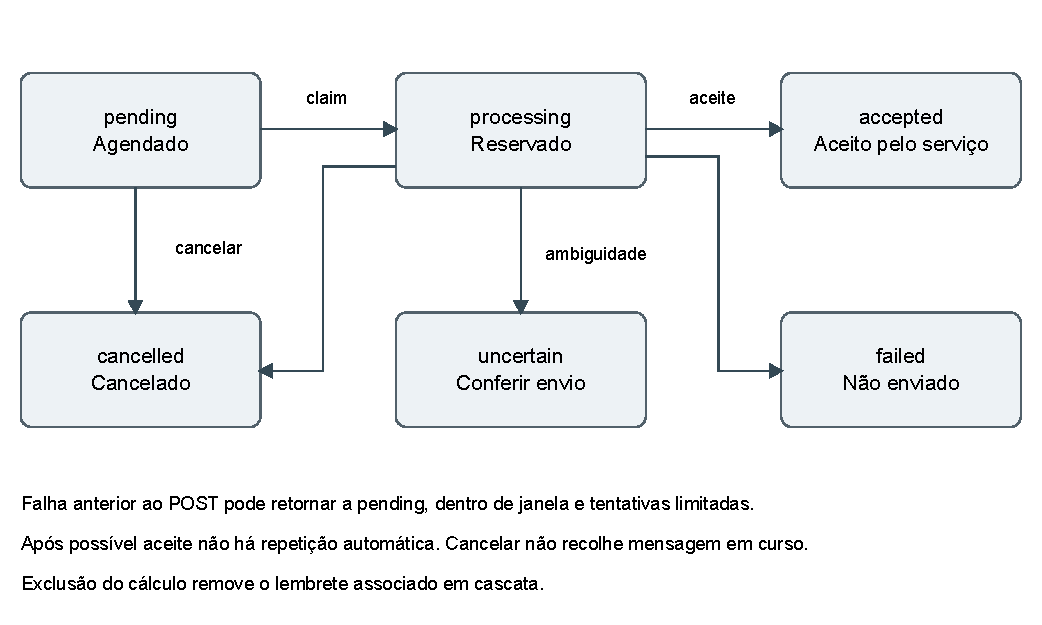
\includegraphics[width=\linewidth,height=.49\textheight,keepaspectratio]{figuras/lembretes.pdf}
\par\smallskip{\fontsize{10}{12}\selectfont Fonte: elaboração para este relatório a partir do código e da documentação do Prazo Claro (2026).}
\end{figure}
O estado accepted significa que o provedor aceitou a mensagem. Não demonstra recebimento, leitura ou execução do ato processual. Timeout ou resposta ambígua após iniciar o POST pode produzir uncertain, sem repetição automática que arrisque duplicação. Cancelamento não recolhe uma mensagem já aceita. As transições e as diferenças entre falha anterior ao envio e resposta incerta possuem testes SQL e de aplicação.

O adaptador Brevo considera sucesso o aceite HTTP 201 com identificador válido, conforme o contrato do provedor \hyperref[ref:BREVO]{(BREVO, s.d.)}. SMTP de autenticação e API de lembretes usam configurações distintas. O conteúdo enviado é mínimo e aponta para a memória privada, cujo acesso continua dependendo da conta proprietária. Não existe e-mail imediato adicional de confirmação do agendamento: a confirmação aparece no site, e a mensagem é prevista para o horário escolhido.

\section{Agendamento e implantação}
\label{section-5-6}
Supabase Cron consulta periodicamente o trabalho elegível e pg\_net chama o dispatcher hospedado. A chamada leva assinatura temporária, operação, timestamp e nonce de uso único. O segredo permanente fica no Vault e no servidor; não é copiado para cabeçalhos persistidos da fila HTTP. O servidor consome a invocação antes de executar. Probe verifica configuração sem obter lembretes nem enviar mensagens.

\begin{figure}[H]\centering
\caption{Implantação e processamento hospedado}
\label{figure-8}
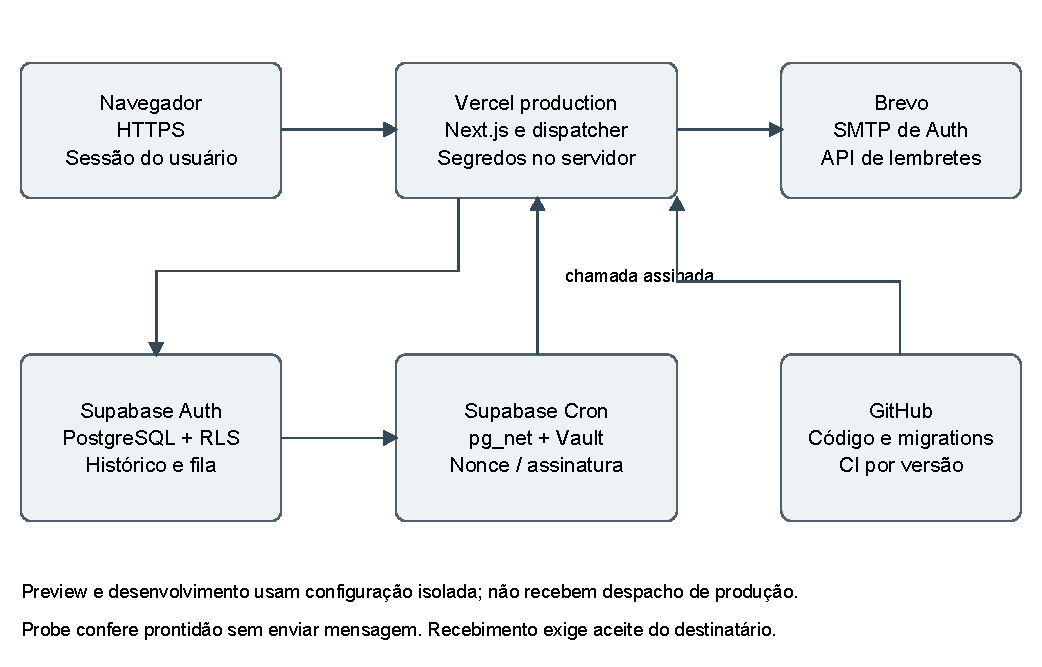
\includegraphics[width=\linewidth,height=.49\textheight,keepaspectratio]{figuras/implantacao.pdf}
\par\smallskip{\fontsize{10}{12}\selectfont Fonte: elaboração para este relatório a partir do código e da documentação do Prazo Claro (2026).}
\end{figure}
A configuração separa desenvolvimento, preview e produção. O preview não recebe credenciais de despacho do banco de produção. O job é preparado inativo; ativação exige diagnóstico recente e pronto. A suspensão operacional combina desativar o agendador e a entrega no servidor. A interface de lembrete informa seu estado sem depender de manter o navegador aberto no processamento hospedado.

A publicação funcional identificada ficou READY na Vercel no domínio https://tg-kezia2.vercel.app. O pacote fonte é gerado por commit, com manifesto e SHA-256, sem .git, dependências, builds ou .env privados. O pacote não contém contas ou dados e não substitui backup do Supabase. Operação ampliada depende de definir responsáveis e exercitar restauração, limites e atendimento.

\section{Estratégia e execução dos testes}
\label{section-5-7}
Os testes unitários verificam marcos, exclusões, travessias, versões, condições de atos e respostas incompletas. Os testes de propriedades exploram invariantes, sem substituir os casos jurídicos de referência. Os testes SQL verificam RLS, proprietário, modos de entrega, concorrência e transições. Os testes de navegador verificam formulário, navegação, exportação e apresentação de estados; alguns usam respostas controladas de API.

Integrações reais locais complementam as simulações: duas contas e acesso anônimo exercitam isolamento; Mailpit permite confirmar e recuperar conta e observar um lembrete sem enviar a terceiros. Os helpers usam identidades efêmeras e limpeza. A política de não reutilizar usuários reais de produção evita transformar um teste automatizado em alteração de dados pessoais.

No caso da página após cadastro, o primeiro teste falhou porque a navegação continuava em /entrar. Depois da implementação, os cenários desktop e celular passaram. Houve ainda uma falha intermediária de seletor de teste, documentada e corrigida sem ser apresentada como defeito do produto. Essa sequência distingue correção de implementação de ajuste do instrumento de verificação.

\chapter{RESULTADOS, DISCUSSÃO E LIMITAÇÕES}
\label{chapter-6}
\section{Funcionalidades observadas}
\label{section-6-1}
O artefato disponibiliza três perfis explícitos, calendário consultável, catálogo inicial de atos, memória, exportação e impressão. Conta, histórico privado e lembrete opcional foram integrados. A aplicação é web responsiva; não foi desenvolvido um aplicativo nativo nem um sistema de análise automática de documentos ou consulta a processos judiciais.

\begin{figure}[H]\centering
\caption{Resultado e avisos na interface publicada}
\label{figure-9}
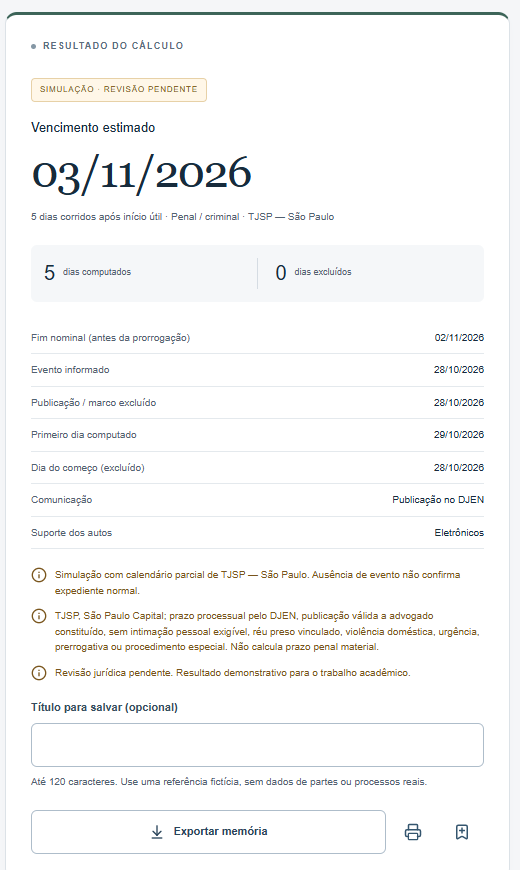
\includegraphics[width=\linewidth,height=.58\textheight,keepaspectratio]{figuras/tela-calculadora.png}
\par\smallskip{\fontsize{10}{12}\selectfont Fonte: captura da aplicação publicada em 23/10/2026, recorte do resultado; acervo do projeto.}
\end{figure}
A figura registra o aplicativo publicado em 23/10/2026. A versão funcional de 24/10 acrescentou a orientação dedicada após cadastro. A captura controlada a seguir mostra essa página sem dados reais de conta; sua existência não comprova a entrega de e-mail em uma execução particular.

\begin{figure}[H]\centering
\caption{Orientação após cadastro em teste controlado}
\label{figure-10}
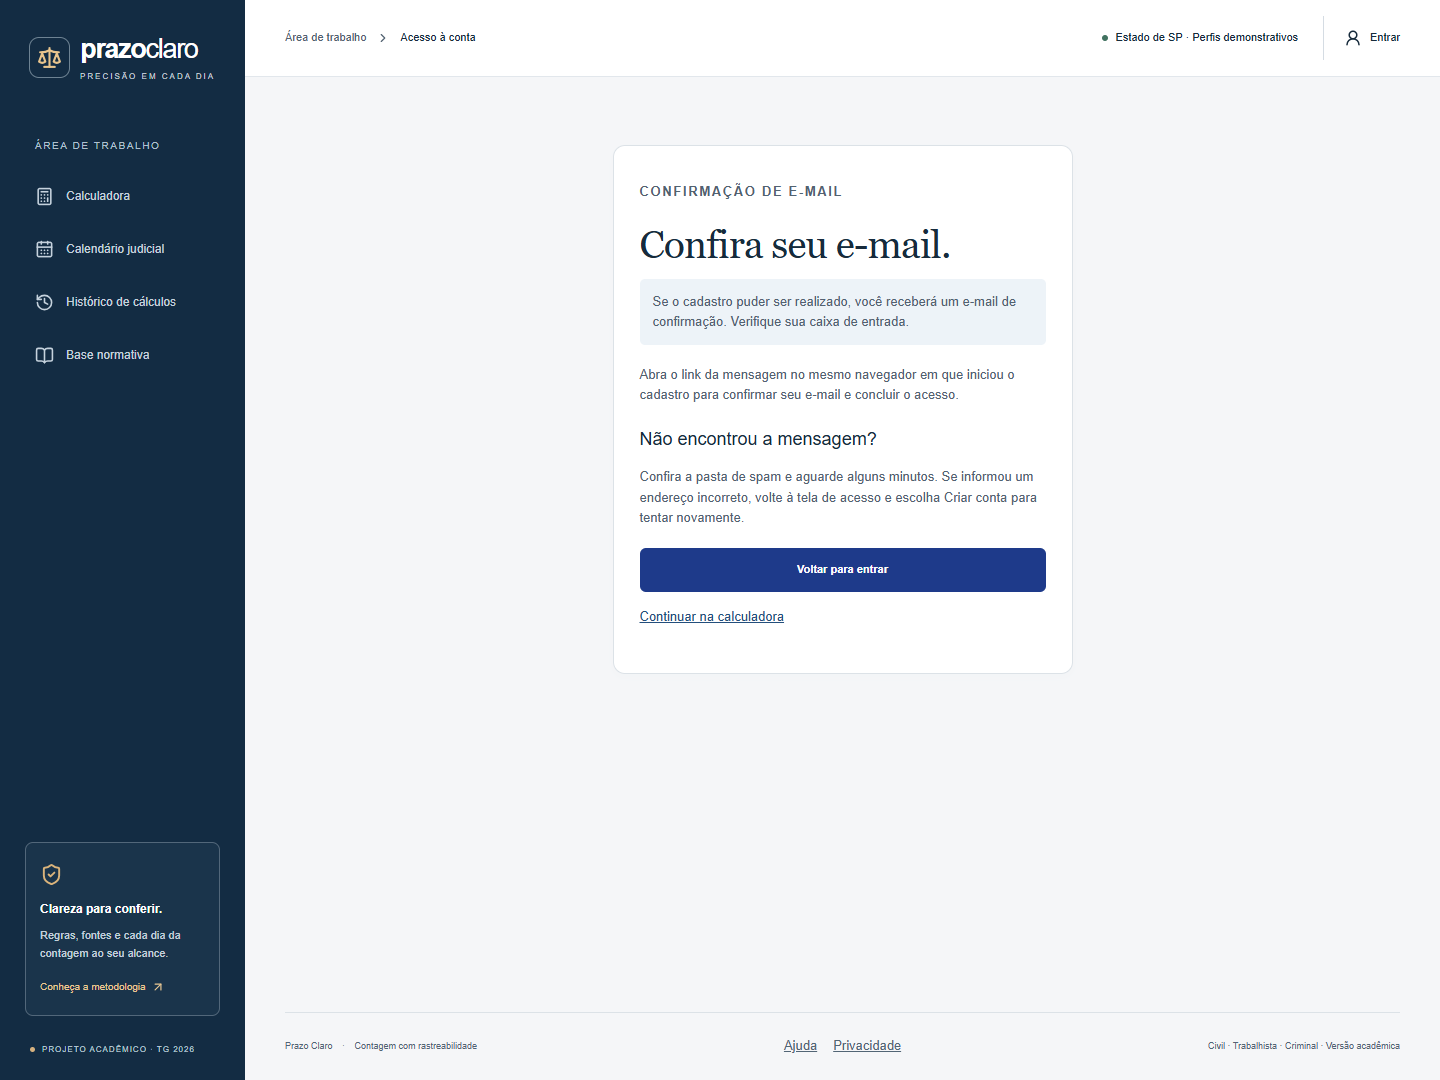
\includegraphics[width=\linewidth,height=.39\textheight,keepaspectratio]{figuras/tela-confirmacao.png}
\par\smallskip{\fontsize{10}{12}\selectfont Fonte: captura de teste controlado da aplicação, 24/10/2026; sem dados reais de conta.}
\end{figure}
\section{Casos de referência e rastreabilidade}
\label{section-6-2}
Os casos a seguir permitem comparar efeitos de perfil e localidade sob os dados demonstrativos. As datas são resultados técnicos das premissas registradas, sujeitos às lacunas do calendário e à revisão jurídica pendente. A mesma entrada numérica não autoriza transferir o resultado entre regimes.

\begin{quadro}[H]\centering
\caption{Casos demonstrativos de referência}
\label{quadro-3}
\begin{singlespace}\fontsize{10}{12}\selectfont
\begin{tabularx}{\linewidth}{|>{\raggedright\arraybackslash}X|>{\raggedright\arraybackslash}X|>{\raggedright\arraybackslash}X|}
\hline
\textbf{Perfil e local} & \textbf{Publicação e duração} & \textbf{Resultado esperado} \\
\hline
Civil TJSP Capital & 06/10/2026; 5 dias úteis & 14/10/2026 \\
\hline
Civil TJSP Santos & 04/09/2026; 1 dia útil & 09/09/2026 \\
\hline
Civil TJSP Capital & 04/09/2026; 1 dia útil & 08/09/2026 \\
\hline
Criminal TJSP Capital, ordinário & 06/10/2026; 5 dias processuais & 13/10/2026 \\
\hline
Trabalhista TRT-2 Capital, ordinário & 17/12/2026; 10 dias úteis & 03/02/2027 \\
\hline
TJSP fora da cobertura temporal & Travessia sem calendário suficiente & Incompleto, vencimento nulo \\
\hline
\end{tabularx}\end{singlespace}
\par\smallskip{\fontsize{10}{12}\selectfont Fonte: elaboração com base nos registros do projeto (2026).}
\end{quadro}
No primeiro caso, a trilha permite conferir 7, 8 e 9 de outubro, a exclusão do fim de semana e de 12 de outubro, e a continuação em 13 e 14. Nos casos de Santos e Capital, a diferença decorre da seleção municipal, não de uma alteração arbitrária da duração. Na travessia trabalhista, a memória identifica os dois componentes anuais e os períodos excluídos.

\section{Resultados automatizados e aceites humanos}
\label{section-6-3}
A CI 40061653068 foi aprovada na versão 9632fd2. O quadro separa verificações de código e banco de observações de uso. Não foi calculado percentual de cobertura de linhas nem desempenho sob carga; contagem de testes aprovados não equivale a essas métricas.

\begin{table}[H]\centering
\caption{Resultados registrados de verificação automatizada}
\label{tabela-1}
\begin{singlespace}\fontsize{10}{12}\selectfont
\begin{tabularx}{\linewidth}{>{\raggedright\arraybackslash}X>{\raggedright\arraybackslash}X>{\raggedright\arraybackslash}X}
\hline
\textbf{Categoria} & \textbf{Aprovados} & \textbf{Arquivos ou observação} \\
\hline
Unitários & 256 & 18 arquivos \\
SQL/pgTAP & 146 & 5 arquivos \\
Navegador E2E & 67 & 1 cenário omitido \\
\hline
\end{tabularx}\end{singlespace}
\par\smallskip{\fontsize{10}{12}\selectfont Fonte: elaboração com base nos registros do projeto (2026).}
\end{table}
Fonte: registros da CI 40061653068 e docs/testing/signup-confirmation-page.md, 24/10/2026. Tipos, lint, formatação e build também foram aprovados na execução identificada. O cenário omitido não foi contado como sucesso. Os totais agregam verificações de diferentes fronteiras e não devem ser somados como uma medida única de qualidade.

O responsável confirmou uso hospedado de Google com retorno conectado, cadastro com recebimento e confirmação de e-mail, entrada da nova conta, recuperação de senha, histórico após recarga e exportação. Esses relatos são aceites operacionais individuais, não uma pesquisa com amostra de usuários. O fluxo de convite possui integração local aprovada; o reensaio completo no ambiente hospedado permanece com aceite próprio.

\section{Situação do lembrete externo}
\label{section-6-4}
O ensaio de 24/10 às 09h foi inconclusivo. O responsável informou que não recebeu a mensagem e excluiu o cálculo, sem lembrar o horário. A fila vazia e a exclusão em cascata explicam a ausência atual do registro, mas não provam se o cancelamento ocorreu antes do horário. Portanto, não se afirma nem entrega bem-sucedida nem uma causa técnica de falha que os dados não permitem demonstrar.

Um novo agendamento foi conferido às 13h44 de 24/10 para 18h de São Paulo, com vencimento estimado em 27/10 e antecedência de três dias. Na conferência, o estado era pending, sem tentativa ou erro, com agendador ativo. Recebimento da mensagem e abertura da memória permaneciam pendentes no corte deste relatório. O registro deve ser mantido até concluir o ensaio; nenhum horário foi antecipado artificialmente para produzir uma evidência de sucesso.

\section{Análise dos objetivos e decisões}
\label{section-6-5}
O primeiro objetivo específico foi atendido tecnicamente pela especificação dos perfis, vocabulário e critérios de aceite, conservando fontes e lacunas. O segundo foi atendido pela separação do motor e pela integração de recursos privados, demonstrada em testes locais e uso hospedado. O terceiro foi atendido no âmbito da verificação técnica e da documentação; validação jurídica, avaliação com participantes e recebimento do novo lembrete continuam sem encerramento.

A principal decisão de projeto foi tornar a insuficiência de dados um resultado explícito. Isso reduz a aparência de cobertura universal, mas exige explicar ao usuário por que uma combinação não gera data. Outra decisão foi preservar motores e snapshots históricos, o que aumenta o custo de manutenção e evita modificar silenciosamente memórias antigas. O uso de serviços gerenciados simplificou a implantação, mas criou dependências de configuração, cotas e disponibilidade externas.

\section{Custos, riscos e validade}
\label{section-6-6}
Não houve levantamento financeiro com faturas nem apontamento completo de horas. Por isso, não se apresenta orçamento executado, retorno de investimento ou economia mensurada. As categorias relevantes são hospedagem, banco e autenticação, envio transacional, eventual domínio, manutenção técnica e revisão jurídica. Planos gratuitos usados na demonstração não constituem garantia permanente de custo zero ou de capacidade para uso institucional.

As ameaças à validade incluem a cobertura parcial dos calendários, a revisão jurídica ausente, a participação concentrada no responsável do projeto e os testes de interface com respostas simuladas. Dependências e regras podem mudar após o corte. A execução em CI amplia a repetibilidade técnica, mas não comprova todas as configurações do ambiente hospedado. Aceite do provedor não prova chegada à caixa de entrada, e ausência de dados após exclusão limita diagnóstico retrospectivo.

A auditoria de dependências contém mitigação específica documentada para braces; saída de sucesso não representa ausência universal de vulnerabilidades. Não foram executados estudo SUS, pesquisa de campo, teste amplo de carga, auditoria independente ou restauração institucional completa. Esses itens não aparecem como gráficos ou tabelas com valores inventados.

\section{Continuidade priorizada}
\label{section-6-7}
O fechamento imediato requer concluir o ensaio externo do lembrete, reensaiar convite hospedado e apresentação, revisar este relatório pela autora e orientação e conferir os anexos acadêmicos exigidos. Em seguida, devem ser priorizados revisão jurídica e levantamento completo das unidades e suspensões do recorte escolhido, antes de expandir tribunais ou afirmar uso profissional.

A evolução técnica inclui política de retenção e atendimento, backup e restauração ensaiados, controle distribuído de abuso, observabilidade e governança de segredos. Funcionalidades como equipes, cadastro completo de processos, administração normativa e novos meios de comunicação dependem de requisitos e testes próprios. Ampliar apenas um seletor visual não resolve essas lacunas.

\chapter{CONCLUSÃO}
\label{chapter-7}
O Prazo Claro materializou uma aplicação web acadêmica de contagem processual com resultados explicáveis e limites identificados. A solução separou a entrada e a seleção de dados do algoritmo determinístico, preservou versões e registrou a trilha de cálculo. A evolução de um recorte civil para perfis criminais e trabalhistas ocorreu mediante condições próprias, sem apresentar um método genérico como válido para qualquer prazo.

Os objetivos de especificação, implementação e verificação técnica foram alcançados no recorte documentado. Conta, histórico e lembrete opcional demonstram integração com serviços externos, enquanto as evidências diferenciam execução local, resposta simulada, uso hospedado e recebimento real. O conjunto de testes aprovado sustenta o comportamento verificado, mas não substitui revisão jurídica ou avaliação ampla com usuários.

A contribuição de engenharia está na combinação de reprodutibilidade, comunicação de incompletude e rastreabilidade entre requisitos, código e evidências. A documentação permite instalar, demonstrar e continuar o artefato sem confundir recursos planejados com recursos existentes. O resultado permanece demonstrativo: calendário completo, aprovação jurídica, fechamento do ensaio externo e preparação institucional para operação ampliada constituem etapas posteriores claramente delimitadas.

\chapter*{REFERÊNCIAS}\phantomsection\addcontentsline{toc}{chapter}{REFERÊNCIAS}
\begin{singlespace}\setlength{\parindent}{0pt}\setlength{\parskip}{12pt}\raggedright
\phantomsection\label{ref:CPP}BRASIL. Decreto-Lei n\textordmasculine{} 3.689, de 3 de outubro de 1941. Código de Processo Penal. Texto compilado. Dispositivos examinados no projeto: arts. 382, 798 e 798-A. Disponível em: \url{https://www.planalto.gov.br/ccivil_03/decreto-lei/del3689.htm}. Acesso em: 24 out. 2026.\par
\phantomsection\label{ref:CLT}BRASIL. Decreto-Lei n\textordmasculine{} 5.452, de 1\textordmasculine{} de maio de 1943. Consolidação das Leis do Trabalho. Texto compilado. Dispositivos examinados no projeto: arts. 775, 775-A e 895, I. Disponível em: \url{https://www.planalto.gov.br/ccivil_03/decreto-lei/del5452.htm}. Acesso em: 24 out. 2026.\par
\phantomsection\label{ref:LEI11419}BRASIL. Lei n\textordmasculine{} 11.419, de 19 de dezembro de 2006. Dispõe sobre a informatização do processo judicial. Art. 4\textordmasculine{}. Disponível em: \url{https://www.planalto.gov.br/ccivil_03/_ato2004-2006/2006/lei/l11419.htm}. Acesso em: 24 out. 2026.\par
\phantomsection\label{ref:CPC}BRASIL. Lei n\textordmasculine{} 13.105, de 16 de março de 2015. Código de Processo Civil. Texto compilado. Dispositivos examinados no projeto: arts. 219, 220, 224, 1.003, \S{} 5\textordmasculine{}, e 1.009. Disponível em: \url{https://www.planalto.gov.br/ccivil_03/_ato2015-2018/2015/lei/l13105.htm}. Acesso em: 24 out. 2026.\par
\phantomsection\label{ref:LGPD}BRASIL. Lei n\textordmasculine{} 13.709, de 14 de agosto de 2018. Lei Geral de Proteção de Dados Pessoais. Texto compilado. Disponível em: \url{https://www.planalto.gov.br/ccivil_03/_ato2015-2018/2018/lei/l13709.htm}. Acesso em: 24 out. 2026.\par
\phantomsection\label{ref:BREVO}BREVO. Send a transactional email. API reference: POST /v3/smtp/email. Documentação oficial, [s.d.]. Disponível em: \url{https://developers.brevo.com/reference/send-transac-email}. Acesso em: 24 out. 2026.\par
\phantomsection\label{ref:CNJ569}CONSELHO NACIONAL DE JUSTIÇA. Resolução n\textordmasculine{} 569, de 13 de agosto de 2024. Altera a Resolução CNJ n\textordmasculine{} 455/2022. Brasília: CNJ, 2024. Disponível em: \url{https://atos.cnj.jus.br/files/original1654112024081566be32b3134ef.pdf}. Acesso em: 24 out. 2026.\par
\phantomsection\label{ref:FATECMANUAL}FACULDADE DE TECNOLOGIA DE CAMPINAS. Manual do Trabalho de Graduação. Atualização de maio de 2024. Campinas: FATEC Campinas, 2024. Disponível em: \url{https://fateccampinas.edu.br/site/wp-content/uploads/2024/10/MANUAL-TG-FATEC-CAMPINAS-ATUALIZADO-MAI_2024.pdf}. Acesso em: 24 out. 2026.\par
\phantomsection\label{ref:FATECPORTAL}FACULDADE DE TECNOLOGIA DE CAMPINAS. Trabalho de Graduação. Portal institucional. Campinas, [s.d.]. Disponível em: \url{https://fateccampinas.com.br/portal/trabalho-de-graduacao/}. Acesso em: 24 out. 2026.\par
\phantomsection\label{ref:SWEBOK}IEEE COMPUTER SOCIETY. Guide to the Software Engineering Body of Knowledge: SWEBOK Guide. Version 4.0a. Hironori Washizaki (ed.). Lançamento indicado na capa: agosto de 2026. Disponível em: \url{https://ieeecs-media.computer.org/media/education/swebok/swebok-v4.pdf}. Acesso em: 24 out. 2026.\par
\phantomsection\label{ref:ISO25010}INTERNATIONAL ORGANIZATION FOR STANDARDIZATION; INTERNATIONAL ELECTROTECHNICAL COMMISSION. ISO/IEC 25010:2023: Systems and software engineering --- Systems and software Quality Requirements and Evaluation (SQuaRE) --- Product quality model. 2. ed. Geneva: ISO, 2023. Resumo público consultado. Disponível em: \url{https://www.iso.org/standard/78176.html}. Acesso em: 24 out. 2026.\par
\phantomsection\label{ref:ASVS}OWASP FOUNDATION. Application Security Verification Standard. Version 5.0.0. 30 maio 2025. Disponível em: \url{https://asvs.owasp.org/}. Acesso em: 24 out. 2026.\par
\phantomsection\label{ref:PROJETO}PRAZO CLARO. Código-fonte, requisitos, decisões e evidências de verificação. Repositório TG-KEZIA2, versão funcional 9632fd2, 24 out. 2026. Acesso privado mediante autorização do proprietário. Disponível em: \url{https://github.com/Eduwilll/TG-KEZIA2}. Acesso em: 24 out. 2026.\par
\phantomsection\label{ref:SUPABASESSR}SUPABASE. Creating a Supabase client for SSR. Documentação oficial, [s.d.]. Disponível em: \url{https://supabase.com/docs/guides/auth/server-side/creating-a-client}. Acesso em: 24 out. 2026.\par
\phantomsection\label{ref:SUPABASERLS}SUPABASE. Row Level Security. Documentação oficial, [s.d.]. Disponível em: \url{https://supabase.com/docs/guides/database/postgres/row-level-security}. Acesso em: 24 out. 2026.\par
\phantomsection\label{ref:TEMPORAL}TC39. Temporal documentation: Temporal.PlainDate. Documentação oficial, [s.d.]. Disponível em: \url{https://tc39.es/proposal-temporal/docs/plaindate.html}. Acesso em: 24 out. 2026.\par
\phantomsection\label{ref:TJSP2813}TRIBUNAL DE JUSTIÇA DO ESTADO DE SÃO PAULO. Provimento CSM n\textordmasculine{} 2.813/2025. Calendário forense do exercício de 2026. Fonte e dispositivos registrados nas fichas jurídicas do projeto. Disponível em: \url{https://esaj.tjsp.jus.br/gcn-frontend-vue/legislacao/find/236794}. Acesso em: 24 out. 2026.\par
\phantomsection\label{ref:TJSPMUN}TRIBUNAL DE JUSTIÇA DO ESTADO DE SÃO PAULO. Relação de feriados municipais para 2026. Conselho Superior da Magistratura. Processo 2018/206016. Diário da Justiça Eletrônico, edição 4334, 25 nov. 2025, p. 3--7. URL abaixo: página 7; demais páginas identificadas na ficha do projeto. Disponível em: \url{https://www.tjsp.jus.br/atcapi/dje/v1/caderno/pagina/download/site?idCaderno=10&idEdicao=4334&idVolume=4334&pagina=7}. Acesso em: 24 out. 2026.\par
\phantomsection\label{ref:TRT2027}TRIBUNAL REGIONAL DO TRABALHO DA 2\textordfeminine{} REGIÃO. Portaria GP n\textordmasculine{} 19, de 12 de agosto de 2026. Calendário de 2027. DEJT administrativo 4537, 14 ago. 2026. Arts. 1\textordmasculine{}--3\textordmasculine{} e anexo. Disponível em: \url{https://basis.trt2.jus.br/bitstream/handle/123456789/18580/2026_port0019_gp.pdf?sequence=3&isAllowed=y}. Acesso em: 24 out. 2026.\par
\phantomsection\label{ref:NEXT}VERCEL. Next.js documentation: Route Handlers. Documentação oficial, [s.d.]. Disponível em: \url{https://nextjs.org/docs/app/getting-started/route-handlers}. Acesso em: 24 out. 2026.\par
\phantomsection\label{ref:WCAG}WORLD WIDE WEB CONSORTIUM. Web Content Accessibility Guidelines (WCAG) 2.2. W3C Recommendation, 12 dez. 2024. Disponível em: \url{https://www.w3.org/TR/WCAG22/}. Acesso em: 24 out. 2026.\par
\end{singlespace}
\appendix
\titleformat{\chapter}[block]{\normalfont\bfseries\fontsize{14}{18}\selectfont}{APÊNDICE \thechapter\space---}{.5em}{}
\chapter{CASOS DE USO DETALHADOS}
\label{chapter-A}
\section{UC01 Realizar simulação pública}
\label{section-A-1}
Ator: visitante. Precondição: aplicação acessível. Fluxo: selecionar perfil e localidade, indicar comunicação, data e duração, declarar contexto quando necessário e solicitar cálculo. O servidor valida e seleciona os catálogos; a tela apresenta memória provisória ou incompleta. Alternativas: campo inválido recebe mensagem associada; combinação não coberta não gera vencimento; falha de rede permite nova tentativa sem salvar resultado fictício. Pós-condição: nenhuma persistência privada é criada automaticamente.

\section{UC02 Selecionar ato do catálogo}
\label{section-A-2}
Ator: visitante ou pessoa autenticada. Precondição: perfil compatível. Fluxo: escolher um dos três atos disponíveis, examinar as condições e confirmar seu enquadramento; a duração fica fixa. Alternativas: condição desconhecida ou excluída, versão inexistente ou duração divergente impedem data final. Ao retornar à quantidade manual, a identificação do ato e sua declaração não são carregadas indevidamente. Pós-condição: memória conserva ficha e versão do ato quando aplicável.

\section{UC03 Exportar memória}
\label{section-A-3}
Ator: pessoa que possui um resultado na tela. Fluxo: examinar avisos e solicitar JSON ou impressão. A saída inclui entrada, marcos, trilha, fontes, versões e estado. Alternativa: resultado incompleto é exportado com vencimento nulo, sem ocultar pendências. Pós-condição: arquivo local ou diálogo de impressão; não há criação automática de conta, certificação ou assinatura de autenticidade.

\section{UC04 Cadastrar e confirmar conta}
\label{section-A-4}
Ator: visitante. Fluxo: informar e-mail e senha, enviar, abrir a página de orientação, receber mensagem e confirmar no mesmo navegador. O retorno válido cria a sessão. Alternativas: erro de validação, limite ou indisponibilidade mantém mensagem compreensível; resposta genérica não revela se a conta existe. Pós-condição: conta confirmada e sessão quando o fluxo é concluído. Receber a mensagem sem abrir o retorno não equivale a estar conectado.

\section{UC05 Entrar ou recuperar acesso}
\label{section-A-5}
Ator: titular da conta. Fluxo: usar e-mail e senha ou Google; no caso de recuperação, solicitar mensagem, abrir o retorno e definir nova senha. Alternativas: credenciais inválidas não concedem sessão; código ausente ou inválido não abre recurso privado; indisponibilidade é distinta de conta inexistente. Pós-condição: sessão verificada ou mensagem de falha. Senha e links não são incluídos nas evidências compartilhadas.

\section{UC06 Aceitar convite}
\label{section-A-6}
Ator: pessoa convidada. Precondição: convite emitido no ambiente correto. Fluxo: receber mensagem, abrir o retorno e concluir definição de senha/acesso. O aplicativo trata o retorno e a sessão do convite. Alternativas: link expirado, uso de destino incorreto ou sessão não estabelecida exigem novo fluxo controlado. Pós-condição: conta acessível quando o convite for aceito. O aceite hospedado deve ser registrado separadamente do teste local.

\section{UC07 Salvar e consultar histórico}
\label{section-A-7}
Ator: pessoa autenticada. Fluxo: salvar entrada calculável com título opcional, abrir histórico, filtrar ramo e navegar pelas páginas. O servidor reexecuta a entrada antes da gravação e fixa o proprietário. Alternativas: sessão ausente retorna 401; cálculo incompleto não é salvo como provisório; memória antiga incompatível conserva original sem recomputação. Pós-condição: cálculo pertencente à conta, com versões e avisos preservados.

\section{UC08 Excluir cálculo}
\label{section-A-8}
Ator: proprietário. Fluxo: selecionar exclusão e confirmar na interface; servidor e RLS restringem a operação. Alternativa: ID de outra conta não permite exclusão. Pós-condição: cálculo removido e lembretes associados removidos em cascata, com atualização da paginação. Não excluir um cálculo usado em ensaio de entrega antes de registrar seu resultado.

\section{UC09 Agendar lembrete}
\label{section-A-9}
Ator: proprietário com e-mail confirmado. Precondições: cálculo elegível salvo, envio futuro e configuração disponível. Fluxo: escolher antecedência e horário, marcar consentimento externo quando exigido e agendar. O servidor resolve destino, fuso e modo. Alternativas: horário passado, geração ativa ou modo incompatível não criam novo envio. Pós-condição: estado Agendado no site. Não há mensagem imediata adicional de confirmação.

\section{UC10 Cancelar e acompanhar lembrete}
\label{section-A-10}
Ator: proprietário. Fluxo: consultar estado, cancelar a geração ou todos os lembretes ativos da conta. Alternativas: tentativa em curso pode já ter sido aceita; estado incerto exige conferência antes de novo pedido. Pós-condição: cancelamento registrado quando cabível, preservando o cálculo. O usuário deve distinguir agendamento, aceite do provedor e recebimento efetivo.

\chapter{DICIONÁRIO DE DADOS}
\label{chapter-B}
\section{Catálogos e histórico}
\label{section-B-1}
\begin{quadro}[H]\centering
\caption{Tabelas públicas de fontes e versões}
\label{quadro-4}
\begin{singlespace}\fontsize{10}{12}\selectfont
\begin{tabularx}{\linewidth}{|>{\raggedright\arraybackslash}X|>{\raggedright\arraybackslash}X|}
\hline
\textbf{Tabela} & \textbf{Campos e restrições essenciais} \\
\hline
legal\_sources & id, title, url, provision, consulted\_at, review\_status e created\_at; descreve origem e revisão. \\
\hline
legal\_rule\_versions & id, rule\_key, version, source\_id, scope JSONB, valid\_from, valid\_until, definition JSONB, review\_status e created\_at; chave única rule\_key/version e FK de fonte com restrição de exclusão. \\
\hline
calendar\_versions & id, calendar\_key, version, court, locality, coverage\_start, coverage\_end, is\_complete, review\_status, snapshot JSONB e created\_at; chave única calendar\_key/version. \\
\hline
deadline\_calculations & id UUID, owner\_id UUID, title opcional, input e result\_snapshot JSONB, status e created\_at; proprietário referencia auth.users com cascata; status persistível provisório. \\
\hline
\end{tabularx}\end{singlespace}
\par\smallskip{\fontsize{10}{12}\selectfont Fonte: elaboração com base nos registros do projeto (2026).}
\end{quadro}
O catálogo ativo do motor está nos arquivos versionados do domínio. A existência das tabelas acima não significa que todas as versões estejam aprovadas e publicadas remotamente. Os campos de JSONB precisam conservar o contrato de leitura; não são prova de integridade criptográfica.

\section{Fila e agendador}
\label{section-B-2}
\begin{quadro}[H]\centering
\caption{Campos operacionais de lembretes}
\label{quadro-5}
\begin{singlespace}\fontsize{10}{12}\selectfont
\begin{tabularx}{\linewidth}{|>{\raggedright\arraybackslash}X|>{\raggedright\arraybackslash}X|}
\hline
\textbf{Grupo} & \textbf{Conteúdo} \\
\hline
Identidade & id, calculation\_id e owner\_id; chaves estrangeiras com cascata. \\
\hline
Programação & due\_date, lead\_days em 0/1/3, send\_hour em 9/12/18, send\_at e time\_zone identificado. \\
\hline
Estado & status em pending, processing, accepted, failed, cancelled ou uncertain; delivery\_mode em local ou brevo. \\
\hline
Concorrência & claim\_token, claimed\_at, attempt\_count limitado e next\_attempt\_at. \\
\hline
Resultado mínimo & accepted\_at, error\_code, snapshot\_metadata e created\_at. \\
\hline
\end{tabularx}\end{singlespace}
\par\smallskip{\fontsize{10}{12}\selectfont Fonte: elaboração com base nos registros do projeto (2026).}
\end{quadro}
reminder\_private.scheduler\_config possui singleton e enabled, com restrição de linha única. scheduler\_invocations possui nonce UUID, issued\_at, operation, created\_at, used\_at, request\_id único, http\_status, completed\_at, timed\_out e summary JSONB. Os dados registram diagnóstico mínimo, com retenção operacional de sete dias para invocações; isso não define a retenção de contas ou históricos.

O schema privado não é exposto como tabela pública da Data API. Wrappers e implementações internas distinguem ações do proprietário e ações exclusivas de serviço. Claim, preparação, conclusão e consumo de invocação não devem ser concedidos ao navegador. Alterações de permissões exigem migrations e testes de isolamento próprios.

\section{Estrutura lógica da memória}
\label{section-B-3}
\begin{quadro}[H]\centering
\caption{Principais elementos de CalculationResult}
\label{quadro-6}
\begin{singlespace}\fontsize{10}{12}\selectfont
\begin{tabularx}{\linewidth}{|>{\raggedright\arraybackslash}X|>{\raggedright\arraybackslash}X|}
\hline
\textbf{Elemento} & \textbf{Significado} \\
\hline
status e dueDate & Provisório com estimativa ou incompleto com vencimento nulo. \\
\hline
input e marcos & Entrada normalizada, evento, publicação, início, primeiro computado e fim nominal quando aplicável. \\
\hline
trace & Datas, counted, ordinal, motivos, sourceIds e fase quando necessária. \\
\hline
sources e warnings & Referências utilizadas e pendências preservadas. \\
\hline
metadata & Versões de motor, regra, calendário, ato e contagem delegada conforme o caso. \\
\hline
snapshot & Cópia do calendário e das fichas de regra/ato pertinentes; componentes anuais opcionais. \\
\hline
\end{tabularx}\end{singlespace}
\par\smallskip{\fontsize{10}{12}\selectfont Fonte: elaboração com base nos registros do projeto (2026).}
\end{quadro}

\chapter{REFERÊNCIA DA API}
\label{chapter-C}
\section{Cálculo público}
\label{section-C-1}
POST /api/calculate recebe JSON de até 16 KB. Datas seguem AAAA-MM-DD; days é inteiro de 1 a 365, sujeito à cobertura. medium identifica suporte dos autos em electronic ou physical, enquanto communication aceita publication ou availability. No civil não se envia context; nos perfis labor e criminal, context é obrigatório e somente ordinary confirmado permite a contagem do recorte.

\begin{quote}\begin{singlespace}\raggedright\ttfamily\footnotesize
\hspace*{0.0em}\{\\
\hspace*{1.0em}"regime": "civil",\\
\hspace*{1.0em}"court": "TJSP",\\
\hspace*{1.0em}"locality": "São Paulo",\\
\hspace*{1.0em}"medium": "electronic",\\
\hspace*{1.0em}"communication": "publication",\\
\hspace*{1.0em}"eventDate": "2026-10-06",\\
\hspace*{1.0em}"days": 5\\
\hspace*{0.0em}\}\\
\end{singlespace}\end{quote}
HTTP 200 retorna CalculationResult diretamente, com status provisional e dueDate 2026-10-14 no exemplo demonstrativo. Um domínio incompleto também usa 200, mas dueDate é null e os motivos são explícitos. JSON inválido ou combinação incompatível usa 400; tamanho excedido usa 413. O resultado completo contém a trilha e não é reduzido aos dois campos citados nesta explicação.

Para apelação civil desta versão, acrescenta-se act com id civil-appeal, version 2026-10-22.demo.1 e eligibility confirmed, usando days 15. Outros IDs são labor-ordinary-appeal e criminal-sentence-clarification. O servidor resolve ficha e duração. Condições unknown ou excluded produzem bloqueio, sem aceitar fonte ou título arbitrário enviados pelo cliente.

\section{Conta e histórico}
\label{section-C-2}
\begin{quadro}[H]\centering
\caption{Rotas de conta}
\label{quadro-7}
\begin{singlespace}\fontsize{10}{12}\selectfont
\begin{tabularx}{\linewidth}{|>{\raggedright\arraybackslash}X|>{\raggedright\arraybackslash}X|}
\hline
\textbf{Método e rota} & \textbf{Contrato principal} \\
\hline
POST /api/auth/signup & email/password; resposta neutra, confirmação exigida e navegação para orientação. \\
\hline
POST /api/auth/login & email/password; sessão SSR por cookie após verificação. \\
\hline
POST /api/auth/logout & Encerra sessão atual; exige mesma origem. \\
\hline
GET /api/auth/session & configured e user; não retorna credenciais. \\
\hline
POST /api/auth/google & Provedor fixo e retorno PKCE; mesma origem. \\
\hline
POST /api/auth/recovery & email; mensagem genérica e retorno controlado. \\
\hline
POST /api/auth/password & password/confirmation; sessão verificada. \\
\hline
GET /auth/callback & Troca de código válido por sessão e destino permitido. \\
\hline
\end{tabularx}\end{singlespace}
\par\smallskip{\fontsize{10}{12}\selectfont Fonte: elaboração com base nos registros do projeto (2026).}
\end{quadro}
Sem configuração, operações dependentes informam indisponibilidade; a consulta de sessão pode informar configured false. Validação e limites podem produzir 400 ou 429; senha inválida não concede sessão. Não se enviam ID de usuário nem destinos externos para escolher a identidade da operação.

GET /api/history aceita page de 1 a 1000, pageSize de 1 a 50, regime opcional e calculationId UUID opcional. Parâmetros desconhecidos ou repetidos são recusados. O retorno contém calculations, asOfDate, timeZone e pagination com totais e navegação. POST recebe input e title opcional, reexecuta e cria resultado provisório com 201. DELETE recebe id do cálculo e restringe a exclusão ao proprietário; não aceita parâmetro para operar como outra conta. Ausência de sessão produz 401.

\section{Lembretes e despacho interno}
\label{section-C-3}
GET /api/reminders consulta estados por cálculos da conta. POST recebe calculationId, leadDays e hour; externalEmailConsent true é obrigatório no modo Brevo e incompatível com o modo local. O servidor escolhe modo e destinatário e responde 201 quando agenda. DELETE cancela geração indicada ou todas as ativas conforme o contrato detalhado. Conflitos de elegibilidade e modo são explícitos, sem fallback para outro provedor.

POST /api/internal/reminders/dispatch recebe operação probe ou dispatch e autenticação de serviço. O protocolo hospedado valida assinatura temporária, timestamp e nonce previamente registrado, consumido uma única vez. Não é uma API para o usuário acionar envio livre. Credenciais e exemplos de assinatura reais não integram este documento. Contratos completos e atualizados permanecem em docs/api e docs/email-reminders-external.md.

\chapter{RASTREABILIDADE E REPRODUÇÃO}
\label{chapter-D}
\section{Requisito, módulo e evidência}
\label{section-D-1}
\begin{quadro}[H]\centering
\caption{Rastreabilidade resumida}
\label{quadro-8}
\begin{singlespace}\fontsize{10}{12}\selectfont
\begin{tabularx}{\linewidth}{|>{\raggedright\arraybackslash}X|>{\raggedright\arraybackslash}X|>{\raggedright\arraybackslash}X|}
\hline
\textbf{Requisito} & \textbf{Implementação principal} & \textbf{Evidência no repositório} \\
\hline
RF01--RF05 & domain/deadlines e application/calculate & multi-regime.md; criminal-sp-expansion.md; labor-2027.md \\
\hline
RF03 & domain/calendars e composição anual & sp-calendars.test.ts; labor-2027.test.ts \\
\hline
RF06 & Memória, exportação e impressão & testing/export-print.md \\
\hline
RF07 & Auth, history e RLS & testing/local-finishing.md; history-organization.md; signup-confirmation-page.md \\
\hline
RF08 & Páginas de calendário e referências & testing/local-finishing.md; release-2026-10-24.md \\
\hline
RF09 & Fila, dispatcher e scheduler & testing/email-reminders.md; reminder-delivery-modes.md; reminders-production.md \\
\hline
RNF01/RNF05 & Motores preservados e snapshot & ADR 0001/0004; testes do domínio e histórico \\
\hline
RNF03/RNF04 & Formulários, rotas e políticas & E2E/Axe, helpers locais e testes SQL \\
\hline
RNF06/RNF07 & Workflows e publicação & CI 40061653068 e testing/release-2026-10-24.md \\
\hline
\end{tabularx}\end{singlespace}
\par\smallskip{\fontsize{10}{12}\selectfont Fonte: elaboração com base nos registros do projeto (2026).}
\end{quadro}
Os caminhos abreviados de evidência textual partem de docs/testing; os arquivos .test.ts partem de tests. A tabela indica onde conferir resultados e limites, sem declarar que cada cenário de navegador percorreu serviços reais.

\section{Instalação e comandos de verificação}
\label{section-D-2}
Obter acesso ao repositório privado ou extrair pacote fonte identificado. Instalar Node e pnpm compatíveis, executar pnpm install --frozen-lockfile e pnpm dev. A calculadora pode funcionar sem Supabase configurado; recursos de conta informam indisponibilidade. O endereço local padrão é http://127.0.0.1:3000.

Para os serviços locais, iniciar Docker e executar pnpm db:start. O helper supabase/scripts/write-local-env.ps1 prepara configuração própria sem sobrescrever arquivo existente. Conferir migration list e aplicar migration up --local quando necessário. Não usar db reset para atualizar uma instalação com dados a preservar. Studio usa 127.0.0.1:54323 e Mailpit 127.0.0.1:54324.

\begin{quote}\begin{singlespace}\raggedright\ttfamily\footnotesize
\hspace*{0.0em}pnpm check\\
\hspace*{0.0em}pnpm build\\
\hspace*{0.0em}pnpm test:e2e\\
\hspace*{0.0em}pnpm db:test\\
\hspace*{0.0em}pnpm db:test:app\\
\hspace*{0.0em}pnpm db:test:invite\\
\hspace*{0.0em}pnpm db:test:recovery\\
\hspace*{0.0em}pnpm db:test:reminders\\
\end{singlespace}\end{quote}
Executar helpers reais sequencialmente no ambiente local isolado e conferir limpeza das fixtures. Lembretes locais exigem configuração própria e watcher ativo; usam Mailpit sem relay externo. Não copiar credenciais de produção para reproduzir testes. Os comandos são instruções de reprodução, não resultados de novas execuções realizadas ao gerar este relatório.

\section{Ensaio de apresentação e aceite}
\label{section-D-3}
Preparar conta de demonstração, títulos fictícios e uma memória PDF já exportada. Em aproximadamente oito a doze minutos de roteiro proposto, apresentar problema e limites, um caso civil, comparação municipal, perfil criminal ou travessia trabalhista, histórico e lembrete. O tempo é estimativa de planejamento, não duração medida de apresentação realizada.

Testar recarga, teclado e tela de celular. Se conexão ou conta falhar, identificar a indisponibilidade e utilizar arquivos preparados, sem chamar uma captura de integração ao vivo. Antes da entrega acadêmica, registrar confirmação de acesso da autora aos materiais, revisão da orientação e resultado do lembrete mantendo o cálculo até o encerramento do ensaio.

\chapter{INSTRUMENTO PROPOSTO DE AVALIAÇÃO}
\label{chapter-E}
\section{Protocolo ainda não executado}
\label{section-E-1}
Este instrumento é uma proposta para avaliação futura e não constitui resultado da pesquisa. Antes de aplicá-lo, definir participantes, consentimento, tratamento de dados e exigências institucionais cabíveis. Utilizar somente casos fictícios e informar a natureza demonstrativa do produto. Não coletar senhas, links de autenticação, número real de processo ou nome de parte.

As tarefas propostas são: calcular o caso civil da Capital; explicar a diferença entre publicação e primeiro dia computado; identificar o aviso de calendário parcial; comparar Santos com Capital; salvar e localizar uma memória; agendar e cancelar um lembrete. Observar conclusão, pedidos de ajuda, interpretação de erros e compreensão do significado de aceite do provedor.

O formulário pode registrar perfil de experiência sem identificação nominal, tarefa, conclusão sem ajuda/com ajuda/não concluída, dificuldade relatada e sugestão. Perguntar se a pessoa compreendeu os limites e onde procuraria os fundamentos. A revisão jurídica deve ser conduzida em trilha separada, por profissional identificado, com casos, fonte e parecer registrados; satisfação com a interface não aprova uma regra.

\section{Critérios futuros de análise}
\label{section-E-2}
Apresentar resultados somente após aplicação real, com número de participantes, método, condições e limites. Se forem usadas escalas padronizadas, citar o instrumento e seguir seu procedimento. Não preencher retrospectivamente pontuações SUS, percentuais de sucesso ou comentários fictícios. Falhas observadas devem gerar requisitos e novos testes, preservando a distinção entre evidência e hipótese.

\chapter{ADEQUAÇÃO ACADÊMICA E MANUTENÇÃO}
\label{chapter-F}
\section{Correspondência com o manual da FATEC}
\label{section-F-1}
A estrutura segue os elementos de TG II descritos no manual institucional de maio de 2024: capa, folha de rosto, resumo, abstract, listas pertinentes, sumário, introdução, fundamentação, método, resultados e discussão, conclusão e referências. Concepção e implementação foram desdobradas em capítulos próprios para documentar a engenharia do artefato \hyperref[ref:FATECMANUAL]{(FATEC CAMPINAS, 2024)}. O projeto não reproduz integralmente o layout gráfico do template.

A composição adota A4, fonte de corpo 12, títulos principais 14, margens superior/esquerda de 3 cm e inferior/direita de 2 cm, entrelinha 1,5 no corpo e recuo de 1,25 cm. Elementos como referências, legendas e resumos usam espaçamento simples. A contagem começa na folha de rosto, e os números aparecem a partir da introdução, no alto à direita. A matriz externa matriz-fatec.md permite conferir cada exigência e a localização.

Folha de aprovação, assinaturas e ficha catalográfica da versão final dependem dos responsáveis institucionais. O portal da FATEC orienta que a biblioteca fornece a ficha e que a aprovação é obtida com a orientação \hyperref[ref:FATECPORTAL]{(FATEC CAMPINAS, s.d.)}. Esses documentos não foram inventados nem preenchidos como aprovados. Dedicatória e agradecimentos são opcionais e devem refletir a manifestação pessoal da autora.

\section{Revisão e governança do documento}
\label{section-F-2}
A autora e a orientação devem revisar título, formulação dos objetivos, termos jurídicos, referências e declaração de assistência tecnológica. A defesa, eventual aprovação e alterações posteriores precisam de registros reais. O relatório é uma versão completa para revisão, não uma afirmação de submissão aceita. A conferência acadêmica não elimina a revisão jurídica indicada no aplicativo.

O conteúdo compartilhado em conteudo.md alimenta Word e LaTeX; os diagramas editáveis são gerados a partir de especificações locais. Atualizar primeiro a fonte e regenerar os artefatos evita versões divergentes. A versão LaTeX mantém capítulos, imagens e referências no mesmo projeto. O guia operacional de dez páginas acompanha o relatório, permitindo consulta rápida durante instalação e demonstração.

\end{document}
